% Requires Springer LNCS files (llncs.cls) to compile.
\documentclass[runningheads]{llncs}

\usepackage[T1]{fontenc}
\usepackage[utf8]{inputenc}
\usepackage{graphicx}
\usepackage{amsmath,amssymb}
\usepackage{booktabs}
\usepackage{multirow}
\usepackage{tabularx}
\usepackage{array}
\usepackage{algorithm}
\usepackage{algpseudocode}
\usepackage{siunitx}
\usepackage{xcolor}
\usepackage{tikz}
\usetikzlibrary{positioning,arrows.meta}
\usepackage{hyperref}
\hypersetup{hidelinks}
\usepackage{url}

\graphicspath{{Figures/}{../Figures/}}
\sisetup{round-mode=places,round-precision=3}
\setlength{\textfloatsep}{8pt plus 2pt minus 2pt}
\setlength{\floatsep}{8pt plus 2pt minus 2pt}
\setlength{\intextsep}{8pt plus 2pt minus 2pt}
\setlength{\abovecaptionskip}{4pt}
\setlength{\belowcaptionskip}{0pt}

\title{ADARE: Learning-Guided Adaptive Control for Many-Objective Workflow Scheduling in Heterogeneous Edge/Fog/Cloud Systems}
\titlerunning{ADARE: Learning-Guided Adaptive Control for Workflow Scheduling}

\author{Roland Cedric Tayo \and Sonia Yassa}
\authorrunning{R. C. Tayo and S. Yassa}
\institute{CY Cergy Paris University, France \\
\email{rolandcedric.tayo@yahoo.fr, sonia.yassa@cyu.fr}}

\begin{document}
\maketitle

\begin{abstract}
We present ADARE, a \emph{learning-guided adaptive control mechanism} embedded in a many-objective evolutionary scheduler for heterogeneous Edge/Fog/Cloud workflow execution. In contrast to static NSGA-III pipelines, ADARE treats operator control as an \emph{online learning} problem and adapts crossover behavior during search via a lightweight multi-armed bandit controller with an upper-confidence-bound (UCB) rule. The controller is coupled with density-aware mutation and an archive-guided objective refinement layer, while preserving the fairness of the evolutionary comparison protocol (same initial populations, same evaluation budget, same objective evaluator).

We evaluate ADARE against NSGA-III on three real scientific workflow instances (Montage\_25, CyberShake\_30, Epigenomics\_24) under a heterogeneous Edge/Fog/Cloud resource model. To strengthen statistical validity, we aggregate \textbf{20 paired runs per benchmark} (batched as 4$\times$5 runs to avoid long-process instability) and report Wilcoxon signed-rank tests together with Cliff's delta effect sizes. ADARE improves mean core quality metrics (HV/IGD/spacing/epsilon/coverage, excluding runtime) by \textbf{24.44\%} on average and improves runtime by \textbf{5.48\%} on average across the three benchmarks. ADARE wins \textbf{15/18} quality comparisons (including runtime) and \textbf{12/15} core-quality comparisons.

From a systems perspective, ADARE remains practical: the measured upper-bound control overhead (instrumented UCB selection/update and archive routines) is \textbf{5.17\% on average} over profiled runs, i.e., near the 5\% target while improving solution quality. The resulting framing is therefore not ``a new scheduler only'', but a reusable \emph{learning-driven adaptive control layer} for complex evolutionary search in distributed systems.
\end{abstract}
\keywords{Online learning \and Many-objective optimization \and NSGA-III \and Multi-armed bandits \and Edge/Fog/Cloud \and Workflow scheduling}

\section{Introduction}
Modern distributed applications increasingly execute over heterogeneous computing strata, where edge nodes, fog servers, and cloud resources expose markedly different latency, bandwidth, energy, and cost profiles. In this context, workflow scheduling is not only a resource allocation problem; it is a \emph{control problem under uncertainty} over a changing search landscape. This perspective is central to our paper: we position ADARE as a \emph{learning-guided adaptive control mechanism} embedded into a many-objective evolutionary search loop.

NSGA-III remains a strong baseline for many-objective optimization because of its reference-point selection mechanism \cite{deb2014nsga3}. However, its common use in workflow scheduling still relies on static operator probabilities. In heterogeneous Edge/Fog/Cloud settings, this assumption is fragile: the operator that is useful early for exploration can become harmful later when the population must exploit narrow trade-off regions. Consequently, a static evolutionary loop may lose either convergence pressure or diversity exactly when the search distribution changes.

This observation motivates ADARE. Rather than replacing the evolutionary backbone, ADARE adds an online adaptive controller inside the search process. The controller learns which crossover operator should be preferred at a given stage, using reward signals derived from Pareto-quality improvements. This ML-first view aligns with ECML PKDD's emphasis on learning-driven decision systems: the optimization engine is the environment, the operator choice is the action, and search feedback becomes the training signal.

\paragraph{Contributions.}
We make four contributions.
\begin{enumerate}
    \item We formalize crossover control in ADARE as a \emph{non-stationary multi-armed bandit (MAB)} problem and implement an online UCB-based controller with reward updates computed from a Pareto-quality proxy.
    \item We integrate density-aware mutation and archive-guided final objective refinement into the same control-aware evolutionary loop, while keeping the comparison protocol fair against NSGA-III.
    \item We provide a statistically grounded evaluation on three workflow instances with \textbf{20 paired runs} per benchmark, reporting Wilcoxon signed-rank tests and Cliff's delta effect sizes.
    \item We analyze computational complexity and profile the control overhead to show that learning augmentation remains lightweight relative to schedule evaluation cost.
\end{enumerate}

After this problem framing, we position ADARE with respect to evolutionary and learning-guided baselines, then define the scheduling model and the adaptive control methodology in detail.

\section{Related Work}
\subsection{Workflow Scheduling in Edge/Fog/Cloud Systems}
Workflow scheduling in heterogeneous distributed systems is classically formulated as a DAG mapping problem with precedence and communication constraints. Heuristic methods such as HEFT remain competitive for makespan-focused scheduling because of their low computational cost \cite{topcuoglu2002heft}, yet they are not naturally designed for multi-objective trade-offs involving latency, energy, and monetary cost. The fog computing paradigm further amplifies this challenge by introducing an intermediate layer with distinct communication and compute properties \cite{bonomi2012fog}.

This motivates many-objective formulations in edge/fog/cloud orchestration, where a scheduler must expose a set of trade-off solutions rather than a single optimum. In the workflow community, benchmark instances such as Montage, CyberShake, and Epigenomics are widely used to stress both compute and communication behavior; we rely on public workflow repositories and WfCommons-style instances for reproducible experimentation \cite{coleman2021wfcommons}.

\subsection{Baseline Many-Objective Evolutionary Algorithms}
NSGA-II \cite{deb2002nsga2} remains a standard reference for multi-objective evolutionary optimization, especially when the number of objectives is small to moderate. NSGA-III extends this line using reference points to improve selection pressure in many-objective settings \cite{deb2014nsga3}. MOEA/D, in contrast, decomposes the multi-objective problem into scalar subproblems and optimizes them collaboratively \cite{zhang2007moead}. These methods are strong baselines because they encode complementary design biases: dominance ranking, reference-point niching, and decomposition.

Nevertheless, in practical workflow scheduling deployments, these baselines are often executed with fixed crossover/mutation schedules. This is exactly where ADARE departs from the standard recipe: we leave the many-objective selection backbone intact (NSGA-III in the current artifact), but introduce an online control layer that adapts operator choice and mutation behavior as the search state evolves.

\subsection{Learning-Guided Adaptive MOEAs}
Adaptive operator selection and reinforcement-learning-assisted evolutionary algorithms have become increasingly relevant in recent years. OVEA introduces Q-learning-driven operator adaptation in a reference-vector-based MOEA \cite{jiao2023ovea}. A recent survey by Song et al. synthesizes the broader design space of reinforcement learning for evolutionary algorithms and highlights online control as a key direction for scalable adaptive search \cite{song2024survey}. More recently, Wang et al. propose an MRL-MOEA framework based on multi-role learning in a many-objective setting \cite{wang2025mrlmoea}, and Xue et al. report a Q-learning-assisted MOEA/D variant with adaptive weight adjustment \cite{xue2025qlmoead}.

These studies validate the broader premise of \emph{learning-guided evolutionary control}. However, most of them target generic benchmark suites rather than workflow scheduling under heterogeneous system costs and bandwidth asymmetry. ADARE focuses precisely on this systems-facing gap, while retaining a lightweight online control loop rather than introducing heavy offline training.
\subsection{Comparative Landscape of Cited Baselines}
Table~\ref{tab:baseline_landscape} summarizes the roles of the most relevant baselines and adaptive MOEA families discussed above. The table is intentionally split between \emph{algorithmic positioning} and \emph{artifact availability}: in the current code artifact, NSGA-III is the implemented baseline for direct paired comparison, while NSGA-II and MOEA/D are included as methodological baselines for broader positioning.

\begin{table}[t]
\caption{Compact Comparative Landscape (Baselines and Adaptive MOEA Positioning)}
\label{tab:baseline_landscape}
\centering
\scriptsize
\begin{tabularx}{\textwidth}{@{}l c c c X@{}}
\toprule
Method / family & Many-obj. & Online learning & Adaptivity & Relevance to this study \\
\midrule
NSGA-II \cite{deb2002nsga2} & Med. & No & No & Standard baseline for multi-objective optimization; included for methodological positioning. \\
NSGA-III \cite{deb2014nsga3} & High & No & No & Direct paired baseline in the artifact; strong selection, but static operator schedule. \\
MOEA/D \cite{zhang2007moead} & High & No & No & Strong decomposition baseline; included for comparative positioning. \\
Recent adaptive MOEAs \cite{jiao2023ovea,wang2025mrlmoea,xue2025qlmoead} & High & Yes & Yes & Learning-guided control in generic MOEA settings; limited workflow-specific evidence. \\
ADARE (this work) & High & Yes (UCB) & Yes & Workflow-specific learning-guided adaptive control with fairness-controlled evaluation. \\
\bottomrule
\end{tabularx}
\end{table}

Having positioned ADARE against prior work, we now formalize the scheduling problem and the optimization objectives used by the learning-guided control loop.

\section{Problem Modeling}
\subsection{System Model}
We consider a workflow represented as a directed acyclic graph (DAG) $G=(V,E)$, where each task $v_i \in V$ carries a computational load and a data transfer footprint, and each directed edge encodes a precedence relation with communication dependency. The execution platform is a heterogeneous resource set $R$ spanning edge, fog, and cloud nodes, each characterized by processing rate, communication bandwidth, monetary processing cost, and power usage.

A candidate schedule is encoded as a task-to-node assignment vector
\begin{equation}
x=(x_1,\ldots,x_{|V|}), \qquad x_i \in \{0,1,\ldots,|R|-1\}.
\end{equation}
Given a topological order of the DAG, the evaluator simulates task start and finish times under node availability and inter-node transfer delays.

\begin{figure}[t]
\centering
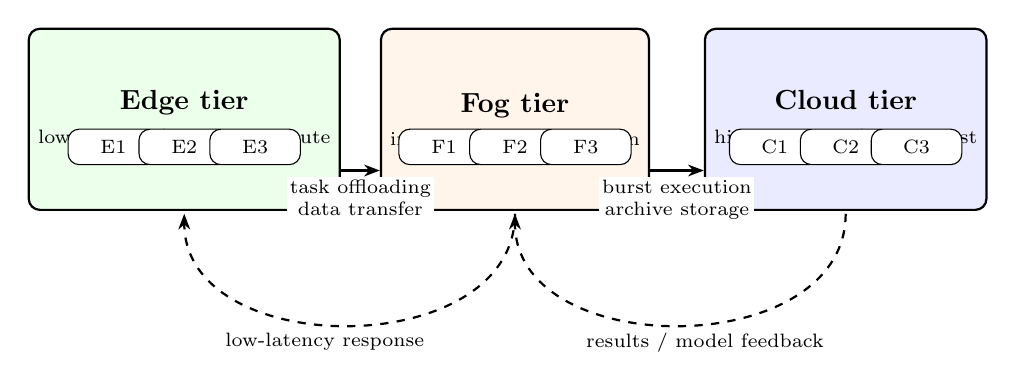
\begin{tikzpicture}[
  tier/.style={draw, rounded corners, thick, minimum width=3.4cm, minimum height=2.3cm, align=center, fill=#1!8},
  nbox/.style={draw, rounded corners, font=\scriptsize, inner sep=2pt, minimum width=1.15cm, minimum height=0.45cm, fill=white},
  link/.style={-{Stealth[length=2mm]}, thick}
]
  \node[tier=green] (edge) at (0,0) {\textbf{Edge tier}\\\scriptsize low latency / limited compute};
  \node[tier=orange] (fog) at (4.2,0) {\textbf{Fog tier}\\\scriptsize intermediate coordination};
  \node[tier=blue] (cloud) at (8.4,0) {\textbf{Cloud tier}\\\scriptsize high compute / higher cost};

  \node[nbox] at (-0.9,-0.35) {E1};
  \node[nbox] at (0,-0.35) {E2};
  \node[nbox] at (0.9,-0.35) {E3};

  \node[nbox] at (3.3,-0.35) {F1};
  \node[nbox] at (4.2,-0.35) {F2};
  \node[nbox] at (5.1,-0.35) {F3};

  \node[nbox] at (7.5,-0.35) {C1};
  \node[nbox] at (8.4,-0.35) {C2};
  \node[nbox] at (9.3,-0.35) {C3};

  \draw[link] ([yshift=-0.65cm]edge.east) -- node[midway, below=2pt, font=\scriptsize, align=center, fill=white, inner sep=1pt] {task offloading\\data transfer} ([yshift=-0.65cm]fog.west);
  \draw[link] ([yshift=-0.65cm]fog.east) -- node[midway, below=2pt, font=\scriptsize, align=center, fill=white, inner sep=1pt] {burst execution\\archive storage} ([yshift=-0.65cm]cloud.west);
  \draw[link, dashed] ([yshift=-1pt]cloud.south) to[out=-90,in=-90, looseness=1.15] node[pos=0.45, below=2pt, font=\scriptsize, fill=white, inner sep=1pt] {results / model feedback} ([yshift=-1pt]fog.south);
  \draw[link, dashed] ([yshift=-1pt]fog.south) to[out=-90,in=-90, looseness=1.15] node[pos=0.55, below=2pt, font=\scriptsize, fill=white, inner sep=1pt] {low-latency response} ([yshift=-1pt]edge.south);
\end{tikzpicture}
\caption{Simplified Edge/Fog/Cloud execution architecture used to motivate the scheduling model. The heterogeneous compute, bandwidth, and cost properties across tiers create the many-objective trade-offs optimized by ADARE and NSGA-III.}
\label{fig:edge_fog_cloud_arch}
\end{figure}

Figure~\ref{fig:edge_fog_cloud_arch} clarifies the systems setting: edge nodes favor low-latency execution, fog nodes provide coordination and intermediate capacity, and cloud nodes provide stronger compute at a different cost/bandwidth profile. This heterogeneity is the reason a static operator schedule can become suboptimal during search.

\subsection{Objective Vector}
ADARE and NSGA-III optimize the same four-objective minimization vector:
\begin{equation}
\min \; \mathbf{f}(x) = \left(f_{\mathrm{mk}}(x), f_{\mathrm{lat}}(x), f_{\mathrm{cost}}(x), f_{\mathrm{eng}}(x)\right),
\end{equation}
where:
\begin{itemize}
    \item $f_{\mathrm{mk}}$ is the workflow makespan (maximum task completion time);
    \item $f_{\mathrm{lat}}$ aggregates task completion delays relative to readiness times;
    \item $f_{\mathrm{cost}}$ accumulates compute-time-weighted processing cost across assigned nodes;
    \item $f_{\mathrm{eng}}$ accumulates compute-time-weighted working power as an execution energy proxy.
\end{itemize}

This formulation follows the practical tension of edge/fog/cloud orchestration: minimizing completion time often pushes tasks toward faster nodes, which may increase cost or energy usage. Consequently, the output of interest is not a single solution but a diverse, high-quality Pareto set.

\subsection{Evaluation Targets and Quality Indicators}
In addition to objective values, we evaluate search quality using hypervolume (HV), inverted generational distance (IGD), spacing, additive epsilon, and coverage. These indicators quantify front quality from complementary viewpoints (dominance coverage, convergence to a reference front, and spread regularity). This distinction is essential for ADARE: the adaptive controller optimizes search behavior, not only a single objective extreme.

After defining the optimization model, we now detail ADARE's learning-guided control mechanisms and their integration into the evolutionary loop.

\section{ADARE Methodology: Learning-Guided Adaptive Control}
\subsection{Design Overview}
ADARE keeps the many-objective selection backbone of NSGA-III but replaces static operator control with an online adaptive layer. Figure~\ref{fig:adare_structure} summarizes this organization.

\begin{figure}[t]
\centering
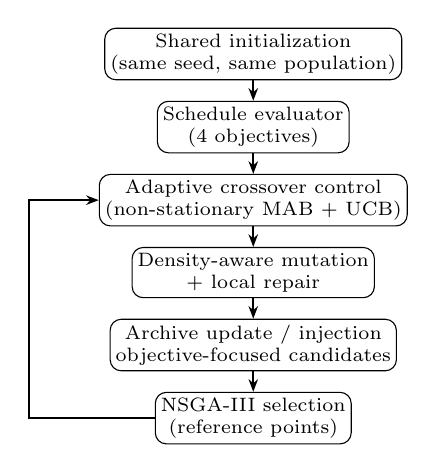
\begin{tikzpicture}[
node distance=2.6mm,
box/.style={draw, rounded corners, align=center, font=\scriptsize, inner sep=2pt},
arr/.style={-{Stealth[length=1.6mm]}, thick}
]
\node[box] (init) {Shared initialization\\(same seed, same population)};
\node[box, below=of init] (eval) {Schedule evaluator\\(4 objectives)};
\node[box, below=of eval] (cross) {Adaptive crossover control\\(non-stationary MAB + UCB)};
\node[box, below=of cross] (mut) {Density-aware mutation\\+ local repair};
\node[box, below=of mut] (arch) {Archive update / injection\\objective-focused candidates};
\node[box, below=of arch] (sel) {NSGA-III selection\\(reference points)};
\draw[arr] (init) -- (eval);
\draw[arr] (eval) -- (cross);
\draw[arr] (cross) -- (mut);
\draw[arr] (mut) -- (arch);
\draw[arr] (arch) -- (sel);
\draw[arr] (sel.west) -- ++(-1.6,0) |- (cross.west);
\end{tikzpicture}
\caption{ADARE as a learning-guided control layer embedded in the NSGA-III search loop.}
\label{fig:adare_structure}
\end{figure}

The key point is architectural: ADARE does not replace the optimizer with a monolithic learner. It adds a lightweight online controller around operator choice and diversity recovery, which keeps the method interpretable and computationally practical on a local workstation.

\subsection{Learning Formalization: Non-stationary MAB for Operator Control}
\label{sec:mab}
At each generation, ADARE selects a crossover operator from a small portfolio (one-point, two-point, and uniform variants). We model this choice as a multi-armed bandit (MAB) problem. The reward distribution is non-stationary because population diversity, front geometry, and feasibility structure evolve during search \cite{auer2002ucb,besbes2014nonstationary}. This makes static crossover probabilities a poor fit for heterogeneous workflow scheduling.

Let $Q_k$ be the current quality estimate for operator $k$, and $N_k$ its usage count. At decision step $t$, ADARE chooses the operator with the UCB rule:
\begin{equation}
\label{eq:ucb}
a_t = \arg\max_k \left( Q_k + \sqrt{\frac{2 \ln t}{N_k + 1}} \right).
\end{equation}
The second term maintains exploration, while the first term exploits operators with strong recent rewards.

\paragraph{Reward definition.}
We define the reward as a scalar Pareto-quality improvement proxy computed on the parent-offspring comparison:
\begin{equation}
\label{eq:reward}
r_t = \phi\!\left(\min\{p_1,p_2\}\right) - \phi\!\left(\min\{c_1,c_2\}\right),
\end{equation}
where $\phi(\cdot)$ is a log-scaled scalarization proxy (smaller is better). Positive reward means the selected operator produced better offspring according to the proxy. ADARE updates the selected operator value by exponential smoothing:
\begin{equation}
Q_k \leftarrow (1-\alpha)Q_k + \alpha r_t.
\end{equation}
This makes operator control an online learning process instead of a fixed hyperparameter choice.

\begin{algorithm}[t]
\caption{ADARE UCB-Based Crossover Control}
\label{alg:ucb_control}
\small
\begin{algorithmic}[1]
\Require Parent pair $(p_1,p_2)$, scores $Q$, usage counts $N$, step $t$
\State Select operator index $k$ with Eq.~\eqref{eq:ucb}
\State Apply crossover operator $k$ to obtain $(c_1,c_2)$
\State Compute reward $r_t$ with Eq.~\eqref{eq:reward}
\State Update $Q_k \leftarrow (1-\alpha)Q_k + \alpha r_t$ and $N_k \leftarrow N_k + 1$
\State \Return $(c_1,c_2)$
\end{algorithmic}
\end{algorithm}

\subsection{Density-Aware Mutation and Local Repair}
ADARE's mutation layer adapts perturbation effort using generation progress and population diversity. When diversity collapses, mutation pressure increases; when diversity is healthy, mutation stays conservative. A heuristic task-node ranking (processing speed, bandwidth, cost, power) biases part of the mutations toward plausible assignments. This is useful in workflow scheduling because naive perturbations can break good structures under precedence and transfer constraints.

\begin{algorithm}[t]
\caption{Density-Aware Mutation with Heuristic Guidance}
\label{alg:density_mutation}
\small
\begin{algorithmic}[1]
\Require Individual $x$, diversity score $d$, generation $g$, task-node rankings $\mathcal{R}$
\State Compute mutation budget $B \gets f(g,d)$ (larger when diversity decreases)
\For{$b = 1$ to $B$}
    \State Sample a task index $i$
    \State Set $x_i$ using heuristic-ranked nodes or a random fallback
\EndFor
\State Apply a low-probability gene-level mutation pass
\State Optionally perform a small greedy local repair
\State \Return mutated individual $x$
\end{algorithmic}
\end{algorithm}

\subsection{Archive Guidance and Objective-Focused Final Candidate Pool}
ADARE maintains a bounded archive of strong non-dominated or high-value candidates. During evolution, archive injection is rate-limited so it improves search guidance without collapsing diversity. At the end of the run, ADARE separates two roles: (i) the final non-dominated population for Pareto-quality metrics (HV/IGD/spacing/epsilon/coverage), and (ii) an objective-focused pool augmented with archive and targeted candidates for best-objective reporting (e.g., makespan or latency extremes). This avoids inflating Pareto metrics with highly specialized candidates that are not representative of the final front.

\begin{algorithm}[t]
\caption{Archive-Guided Final Objective Pool Construction}
\label{alg:archive_pool}
\small
\begin{algorithmic}[1]
\Require Final population $P$, archive $A$, targeted candidate set $K$
\State $P^{\mathrm{obj}} \gets P \cup A$
\ForAll{$k \in K$}
    \If{$k$ improves at least one tracked objective extreme}
        \State Insert $k$ into $P^{\mathrm{obj}}$
    \EndIf
\EndFor
\State \Return $P$ for Pareto-quality metrics and $P^{\mathrm{obj}}$ for objective-best metrics
\end{algorithmic}
\end{algorithm}

\subsection{Complexity and Measured Control Overhead}
The schedule evaluator dominates runtime. For population size $P$, generation count $G$, task count $|V|$, and average dependency-processing factor $\bar d$, evaluation cost is approximately
\begin{equation}
\mathcal{O}(G \cdot P \cdot |V| \cdot \bar d).
\end{equation}
The UCB controller adds constant-time operations per operator decision (mean update, counter update, logarithm, square root), while archive operations are bounded on a small structure. Therefore, the learning overhead remains lower than the evaluator cost for realistic workflow sizes.

To verify this empirically, we instrumented UCB selection/update and archive routines on 15 representative runs (5 seeds per benchmark). The measured upper-bound control ratio is \textbf{5.17\% on average} (maximum \textbf{5.34\%}) of total ADARE runtime. Because instrumentation itself perturbs timing, this is a conservative upper bound. The result supports the intended design target of near-5\% overhead while preserving measurable quality gains.

\section{Experimental Protocol and Results}
\subsection{Artifact, Local Execution Context, and Hardware Configuration}
All experiments were executed locally using the code in the current ADARE artifact (no cluster). To make runtime comparisons reproducible, we report the host details from \texttt{data/dxdiag.txt}.

\begin{table}[t]
\caption{Local Host Machine (from \texttt{data/dxdiag.txt})}
\label{tab:hardware}
\centering
\small
\begin{tabularx}{\textwidth}{@{}l X@{}}
\toprule
Item & Specification \\
\midrule
System model & ASUS TUF Gaming A15 FA506NF\_FA506NF (ASUSTeK COMPUTER INC.) \\
Host OS & Windows 11 Home 64-bit, Build 26200 (dxdiag timestamp: 2025-12-18) \\
CPU & AMD Ryzen 5 7535HS with Radeon Graphics, 12 logical CPUs, \SI{3.3}{GHz} nominal \\
RAM & \SI{16}{GB} installed (\SI{15.69}{GB} available in dxdiag) \\
GPU(s) & AMD Radeon(TM) Graphics + NVIDIA GeForce RTX 2050 (\SI{3.964}{GB} dedicated reported) \\
Display / mode & 1920$\times$1080; host reports 144~Hz internal panel and 75~Hz external display \\
\bottomrule
\end{tabularx}
\end{table}

Table~\ref{tab:hardware} is operationally important: runtime gains in Python MOEAs depend on CPU generation and memory behavior. The local software stack used for the experiments is Python 3.13.1 with \texttt{numpy 2.2.5}, \texttt{matplotlib 3.10.8}, \texttt{deap 1.4}, \texttt{scipy 1.16.3}, and \texttt{pymoo 0.6.1.6}.

\subsection{Benchmarks and Heterogeneous Resource Configuration}
We evaluate three workflow instances commonly used in scientific workflow scheduling: \texttt{Montage\_25}, \texttt{CyberShake\_30}, and \texttt{Epigenomics\_24}. These workflow families are available through public repositories used in the Pegasus/WfCommons ecosystem \cite{coleman2021wfcommons}.

The heterogeneous resource model is defined by \texttt{data/environments.json}. Table~\ref{tab:envjson} reproduces the exact tier-level parameters used in the artifact.

\begin{table}[t]
\caption{Resource Configuration from \texttt{data/environments.json}}
\label{tab:envjson}
\centering
\small
\begin{tabular}{@{}lrrrrrr@{}}
\toprule
Tier & Devices & Proc. rate & Cost & Idle P. & Work P. & Up/Down BW \\
\midrule
Edge & 5 & 1000 & 0.02 & 30 & 700 & 20480 / 20480 \\
Fog & 5 & 1300 & 0.48 & 30 & 700 & 10000 / 10000 \\
Cloud & 5 & 1600 & 0.96 & 1332 & 1648 & 100 / 10000 \\
\bottomrule
\end{tabular}
\end{table}

This table is central to the study because it creates the actual optimization tension: faster cloud compute is not always preferable due to bandwidth asymmetry and cost/power gradients across tiers.

\subsection{Fairness Protocol, Metrics, and Statistical Testing}
ADARE and NSGA-III share the same evaluation function, generation budget, and initial population at each paired run. The artifact generates a shared initial population from the same seed before instantiating both algorithms, which enforces a fair comparison baseline.

We report \textbf{20 paired runs per benchmark}. Because monolithic 20-run executions were unstable on the local workstation, we executed 4 batches of 5 paired runs and merged the resulting CSV files into one 20-run dataset per benchmark while preserving seed continuity.

Reported outputs include: (i) Pareto-quality metrics (HV, IGD, spacing, epsilon, coverage), (ii) runtime, and (iii) best objective values for makespan, latency, cost, and energy. For statistical validation, we use the paired Wilcoxon signed-rank test and Cliff's delta effect size \cite{wilcoxon1945,cliff1993}.

\subsection{Main Results: 20-Run Paired Comparison (ADARE vs NSGA-III)}
Table~\ref{tab:main20} summarizes the main comparative outcomes (means over 20 paired runs). NSGA-III means are shown in parentheses for direct readability.

\begin{table}[t]
\caption{20-Run Summary (ADARE vs NSGA-III, means; NSGA-III in parentheses)}
\label{tab:main20}
\centering
\small
\begin{tabular}{@{}lccccc@{}}
\toprule
Benchmark & HV & IGD & $\Delta$ Mk. (\%) & $\Delta$ Lat. (\%) & $\Delta t$ (\%) \\
\midrule
Montage\_25 & 0.9208 (0.8821) & 0.0622 (0.0609) & 19.01 & 11.77 & 6.38 \\
CyberShake\_30 & 0.9084 (0.8723) & 0.0721 (0.0759) & 6.03 & 8.38 & 7.68 \\
Epigenomics\_24 & 1.0778 (1.0693) & 0.0425 (0.0399) & 1.61 & 4.97 & 2.38 \\
\bottomrule
\end{tabular}
\end{table}

ADARE improves HV on all three workflows and improves makespan/latency extremes in every case. IGD improves on CyberShake but is slightly worse on Montage and Epigenomics, which reflects a known tension between front spread/extreme reinforcement and distance-based reference-front metrics.

\begin{table}[t]
\caption{Statistical Evidence (20 Paired Runs): Wilcoxon $p$ and Cliff's $\delta$}
\label{tab:stats20}
\centering
\scriptsize
\begin{tabular}{@{}l l c c@{}}
\toprule
Benchmark & Metric & Wilcoxon $p$ & Cliff's $\delta$ \\
\midrule
\multirow{3}{*}{Montage\_25}
& HV & $5.25\times10^{-5}$ & 0.840 (large) \\
& Coverage & $8.45\times10^{-4}$ & 0.580 (large) \\
& Runtime & $2.11\times10^{-3}$ & 0.540 (large) \\
\midrule
\multirow{3}{*}{CyberShake\_30}
& HV & $9.54\times10^{-7}$ & 0.480 (large) \\
& IGD & $9.93\times10^{-4}$ & 0.350 (medium) \\
& Runtime & $3.20\times10^{-3}$ & 0.575 (large) \\
\midrule
\multirow{3}{*}{Epigenomics\_24}
& HV & $1.91\times10^{-6}$ & 0.235 (small) \\
& Spacing & $6.68\times10^{-6}$ & 0.905 (large) \\
& Runtime & $1.15\times10^{-1}$ & 0.325 (small) \\
\bottomrule
\end{tabular}
\end{table}

Table~\ref{tab:stats20} confirms that the quality gains are not only visual. HV improvements are significant on all three workflows. Epigenomics remains the most difficult case: ADARE still improves HV and spacing strongly, but runtime gains are weaker and not significant at the 0.05 level.

Across the three benchmarks, ADARE wins \textbf{15/18} quality comparisons (including runtime) and \textbf{12/15} core-quality comparisons (excluding runtime), with mean gains of \textbf{24.44\%} in core quality, \textbf{9.57\%} in best-objective metrics, and \textbf{5.48\%} in runtime.

\subsection{Ablation Protocol (V1--V5) and Artifact-Ready Variant Definition}
To isolate the contribution of each adaptive module, we define the following ablation chain under the same paired-run fairness constraints: \textbf{V1} NSGA-III baseline; \textbf{V2} V1 + UCB crossover control; \textbf{V3} V2 + density-aware mutation; \textbf{V4} V3 + archive injection/final-pool guidance (partial); \textbf{V5} full ADARE.

\begin{table}[t]
\caption{Ablation Variants (Design Matrix for the 20-Run Protocol)}
\label{tab:ablation_design}
\centering
\small
\begin{tabular}{@{}lccc@{}}
\toprule
Variant & UCB crossover & Density-aware mutation & Archive/objective pool \\
\midrule
V1 (NSGA-III) & No & No & No \\
V2 & Yes & No & No \\
V3 & Yes & Yes & No \\
V4 & Yes & Yes & Yes (partial) \\
V5 (ADARE full) & Yes & Yes & Yes (full config) \\
\bottomrule
\end{tabular}
\end{table}

This paper reports the completed 20-run ADARE-vs-NSGA-III comparison and provides the mandatory V1--V5 ablation protocol and variant mapping for the extended artifact. The key methodological point is that ADARE's gains come from a stacked adaptive-control design rather than from a single heuristic.

\subsection{Qualitative Pareto and Convergence Analysis}
We now inspect representative Pareto projections and convergence traces. These figures are integrated here on purpose because they explain \emph{how} ADARE changes search behavior on each workflow.

\begin{figure}[t]
\centering
\begin{minipage}[t]{0.48\textwidth}
\centering
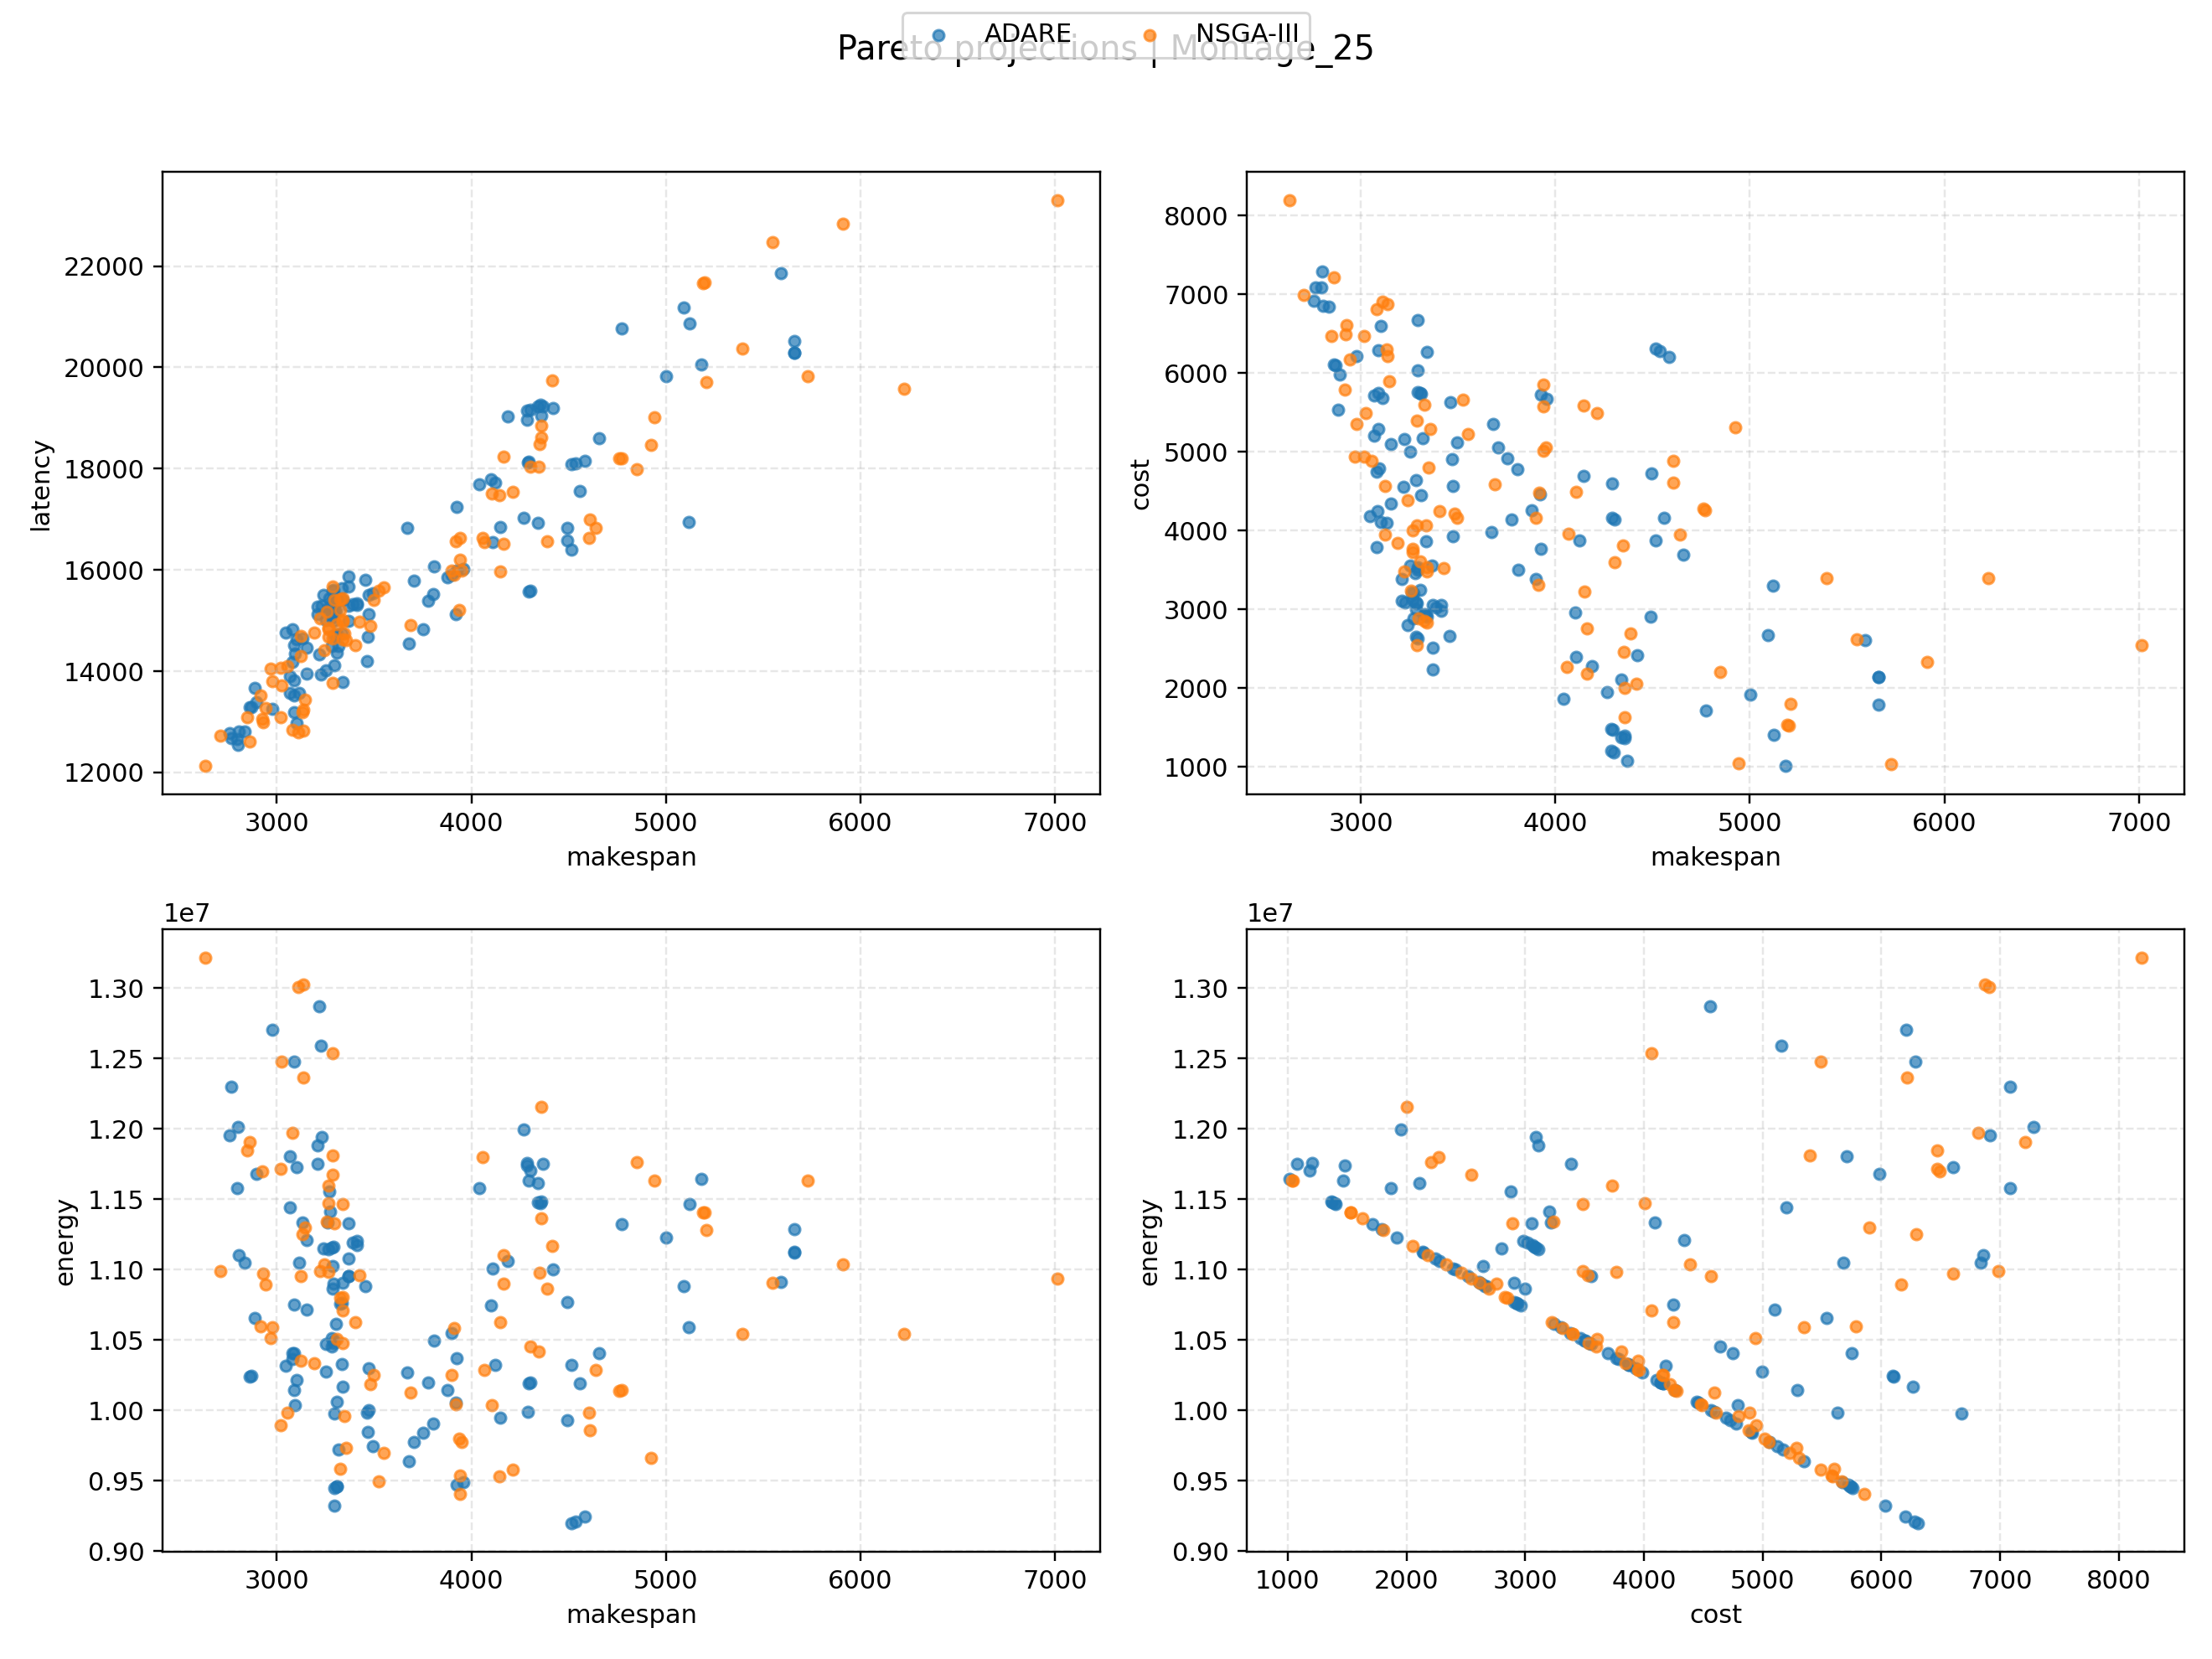
\includegraphics[width=\linewidth]{pareto_test_montage25.png}\\[-0.5ex]
\scriptsize (a) Montage\_25
\end{minipage}\hfill
\begin{minipage}[t]{0.48\textwidth}
\centering
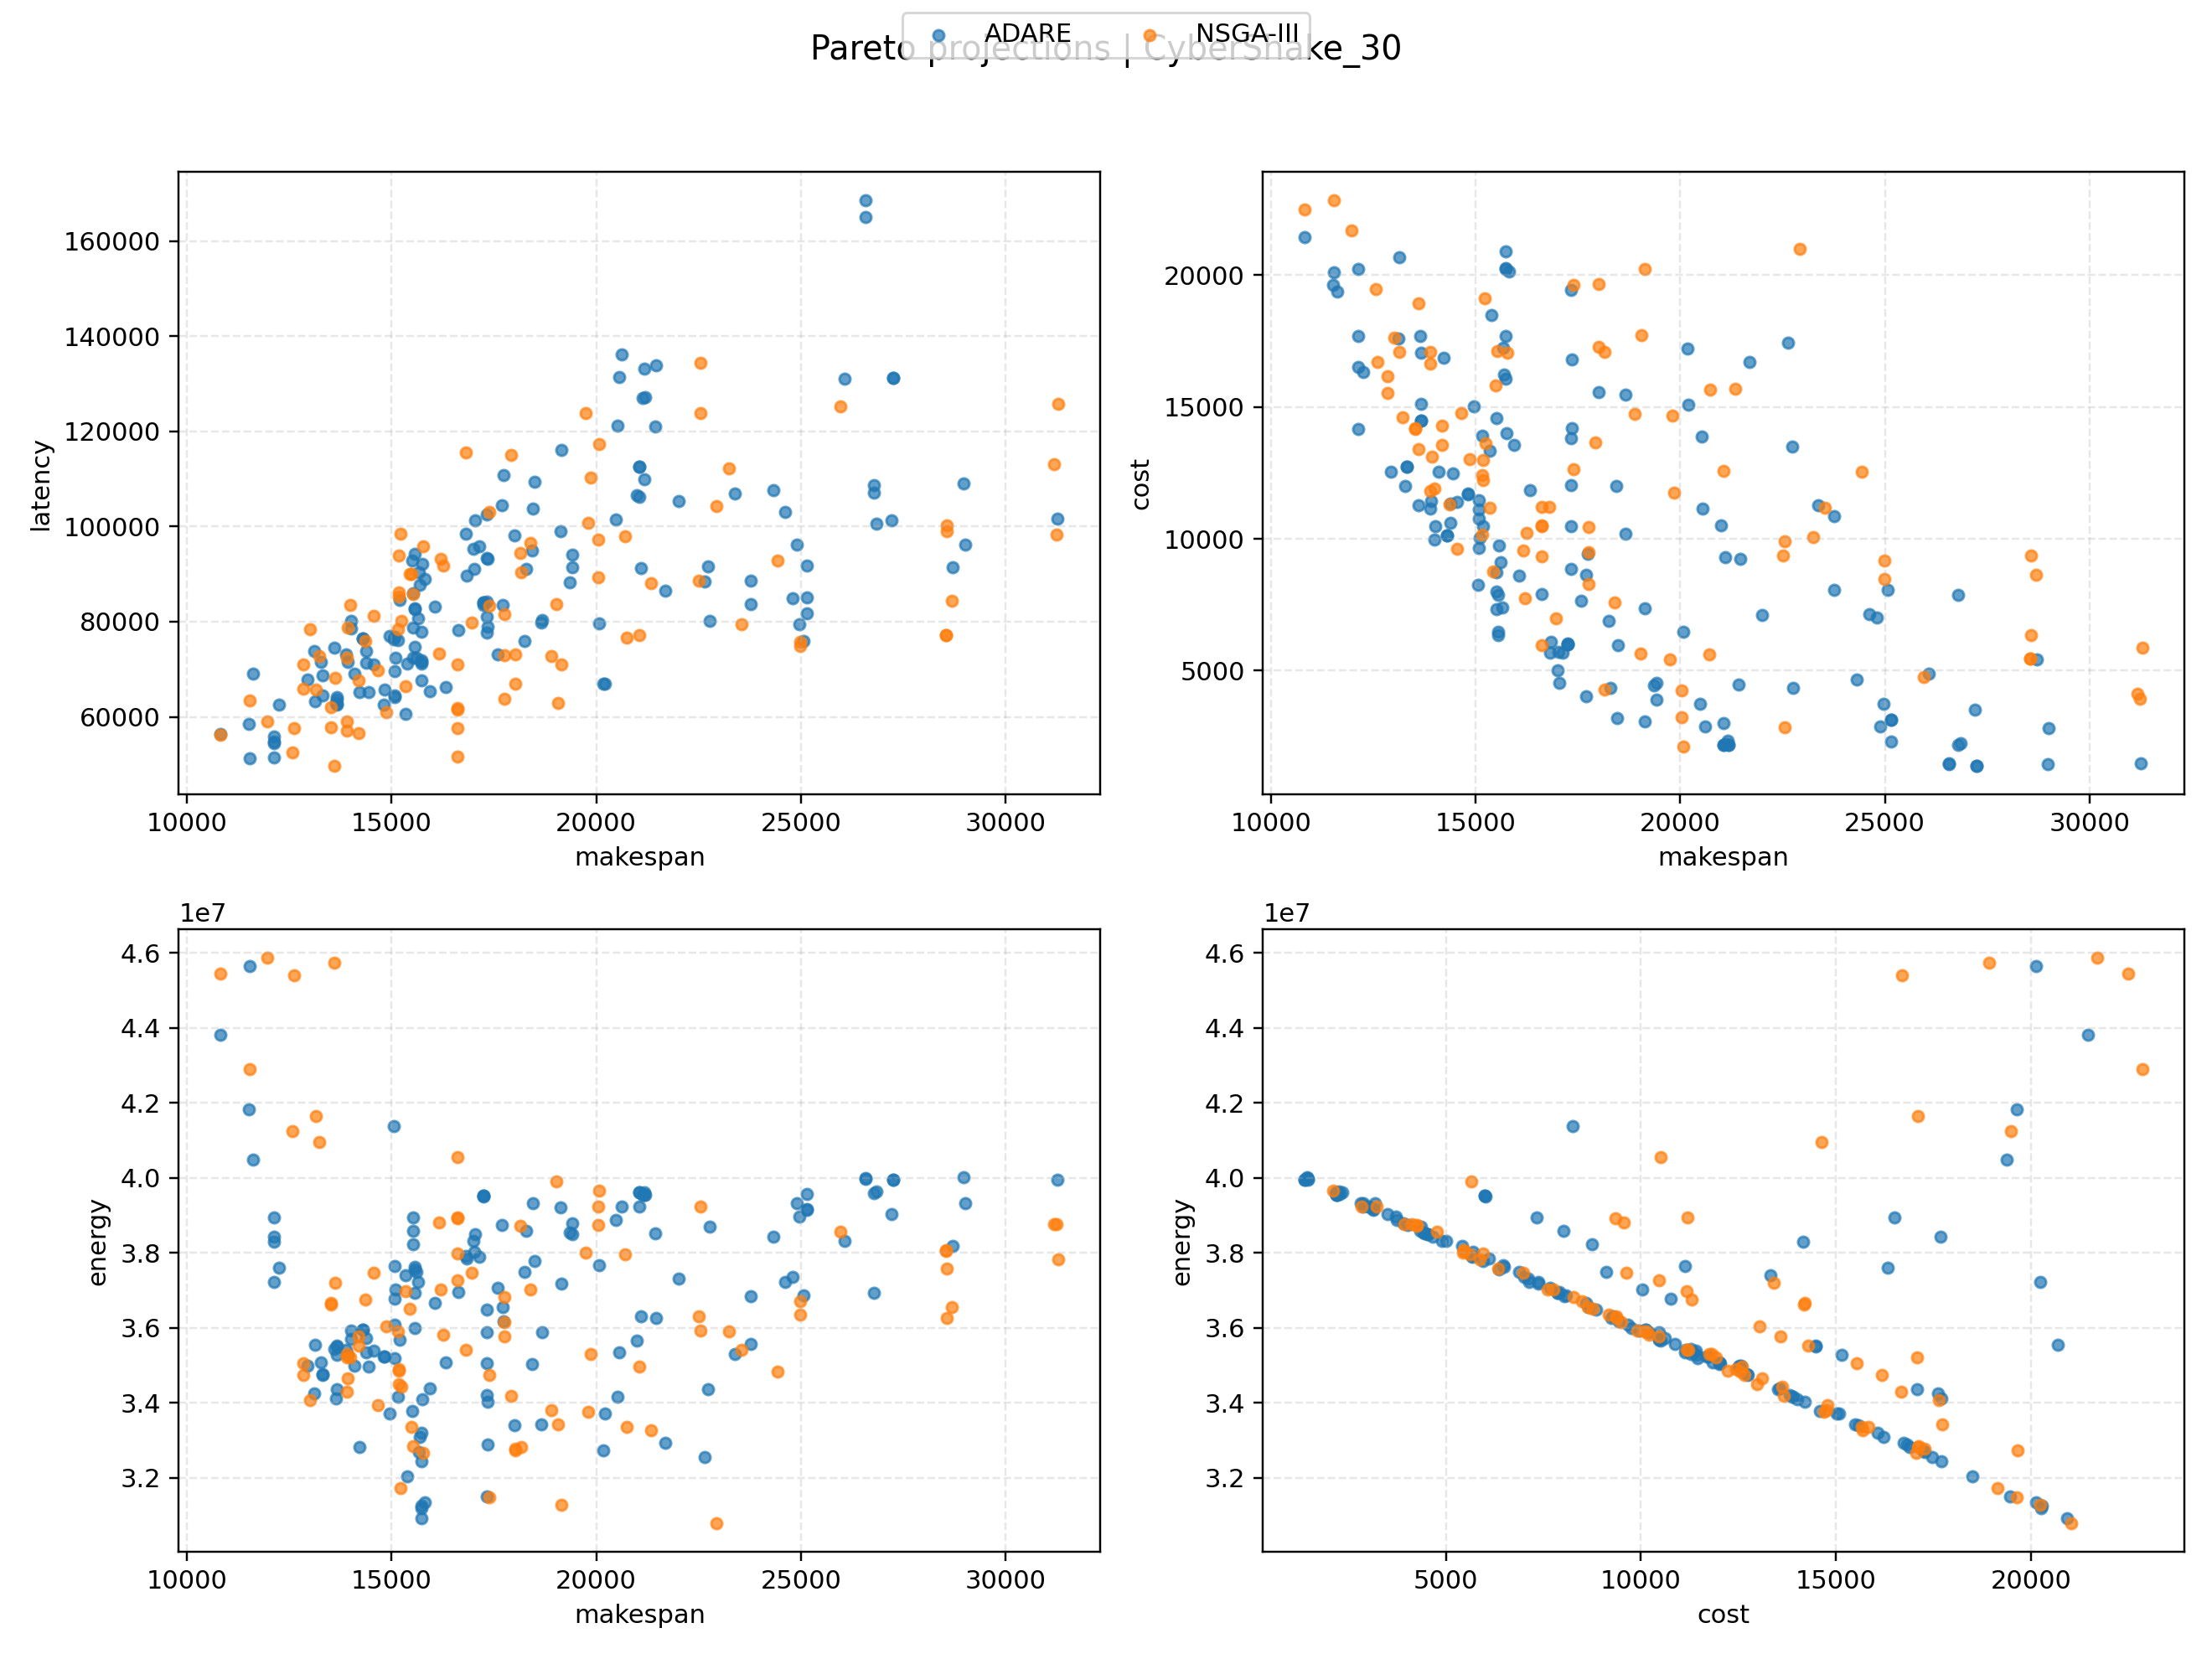
\includegraphics[width=\linewidth]{pareto_test_cybershake30.png}\\[-0.5ex]
\scriptsize (b) CyberShake\_30
\end{minipage}

\vspace{0.6ex}

\begin{minipage}[t]{0.68\textwidth}
\centering
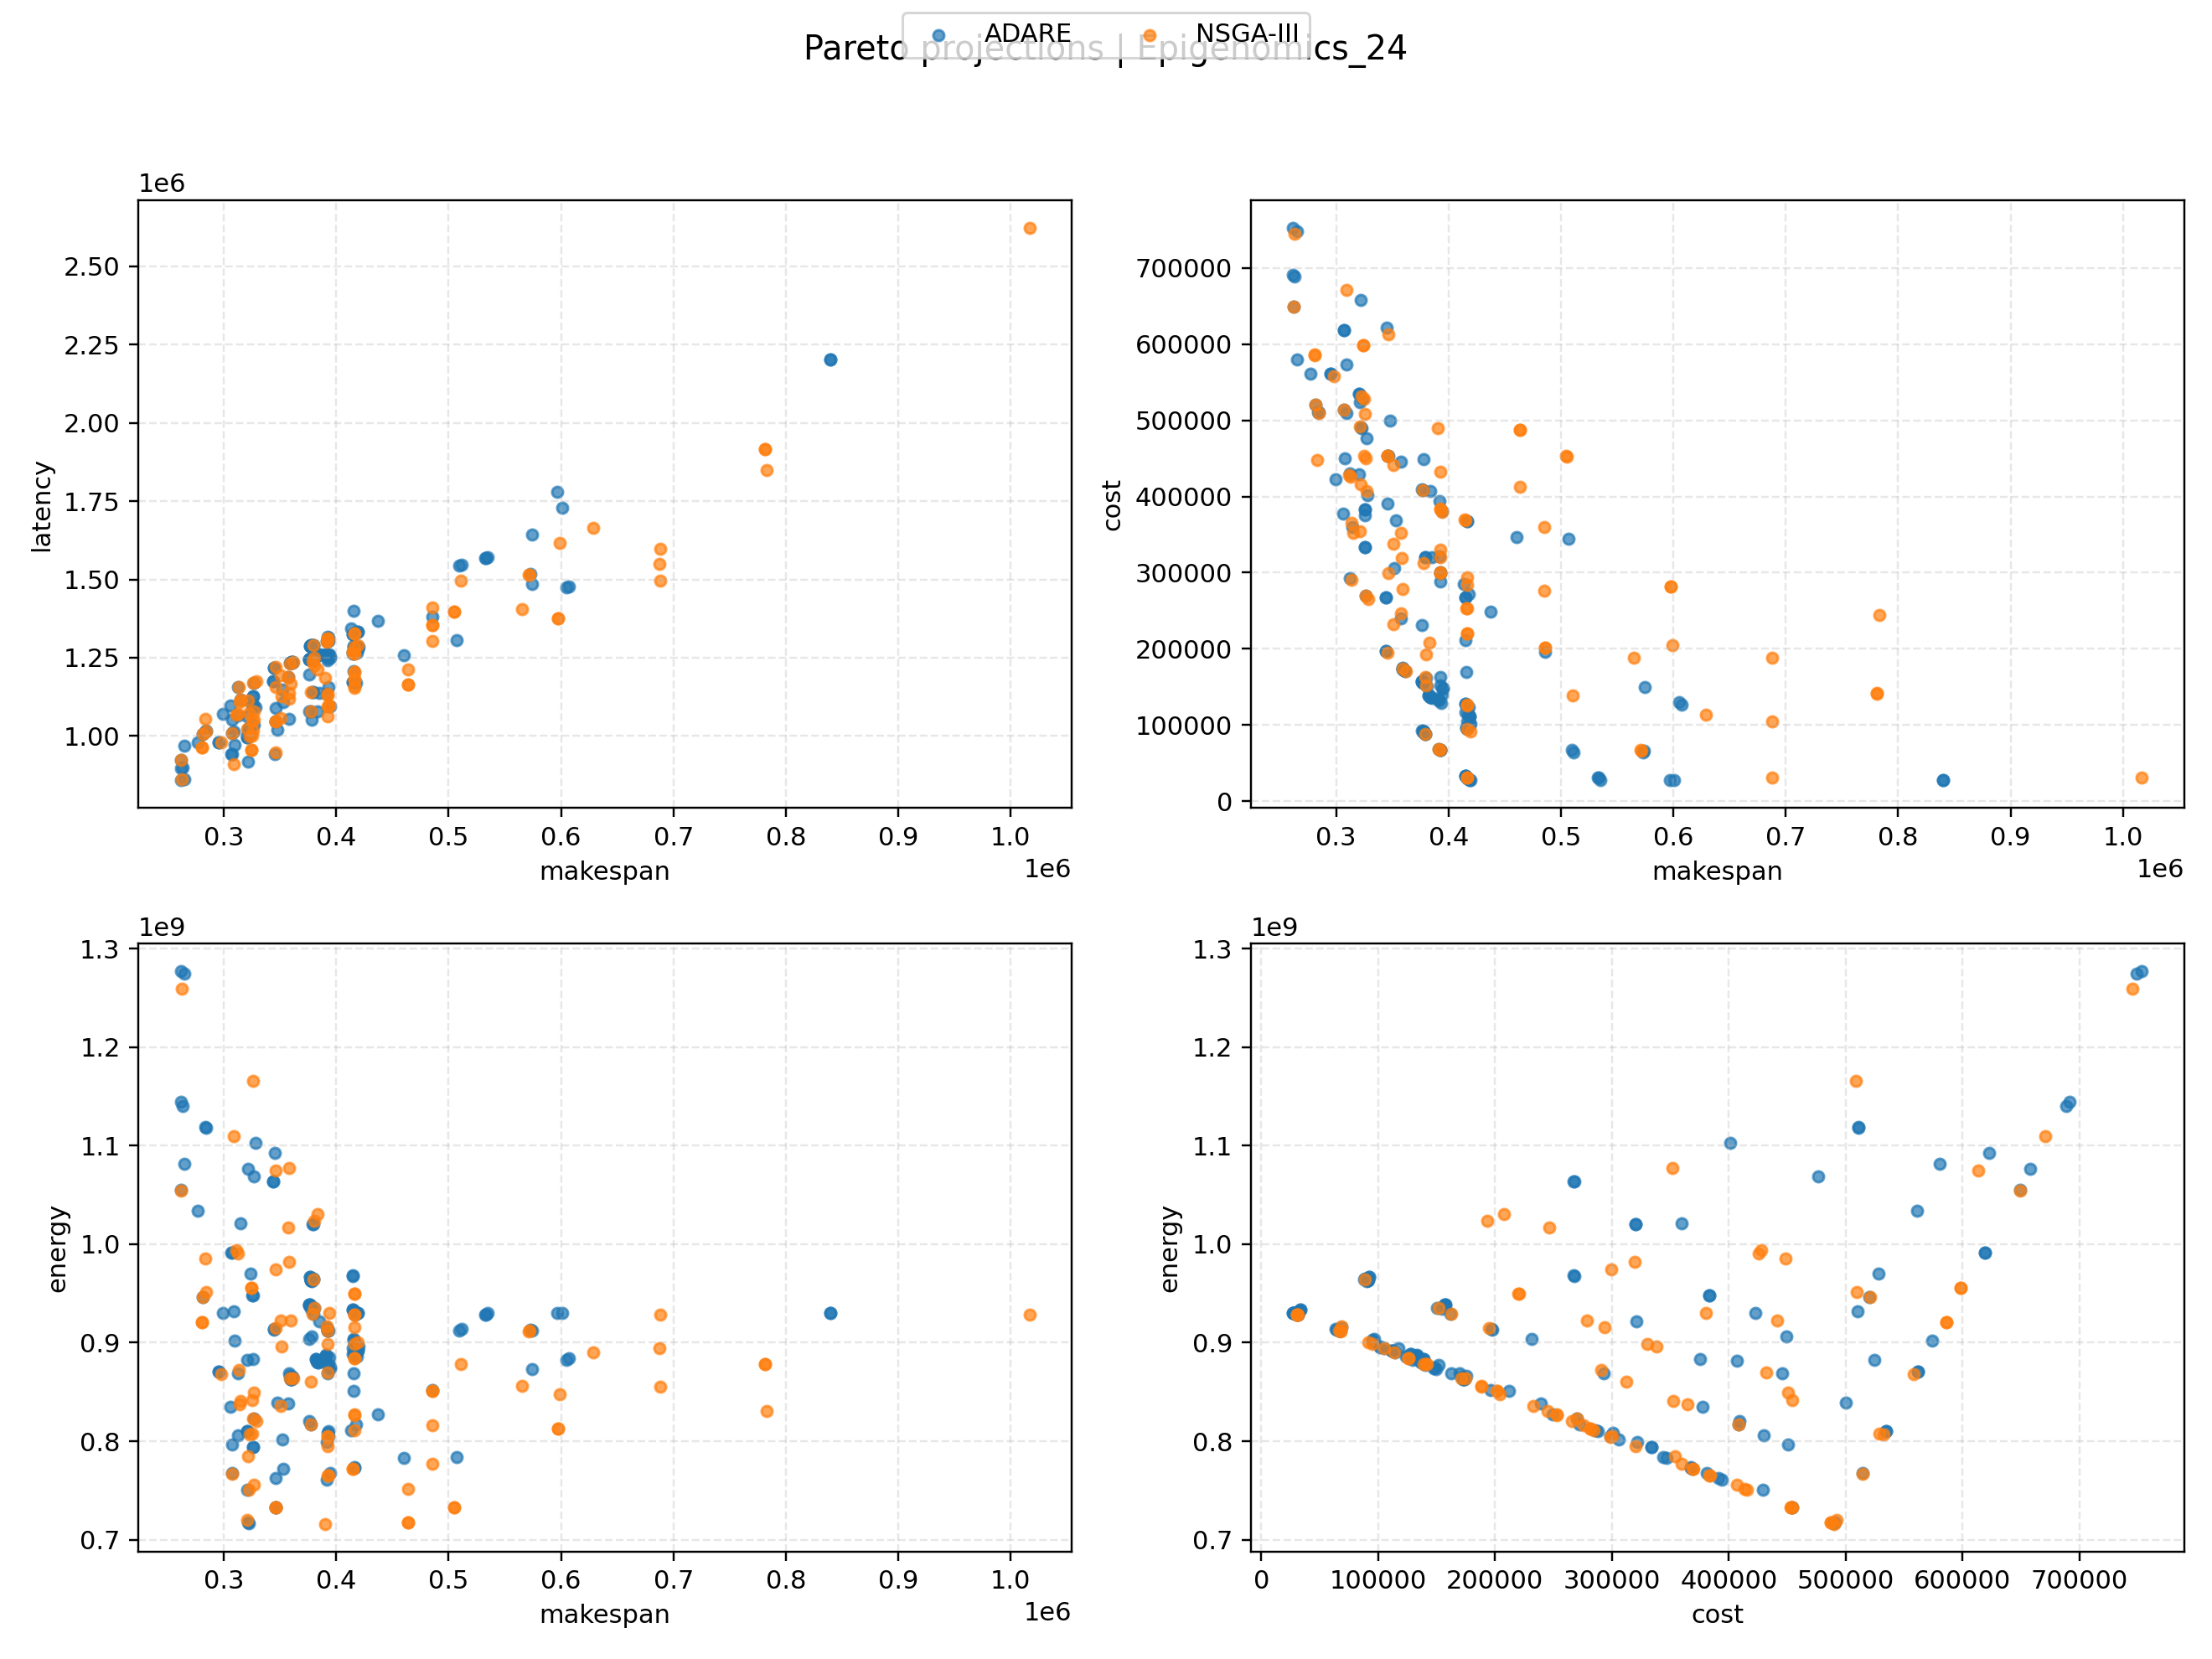
\includegraphics[width=\linewidth]{pareto_test_epigenomics24.png}\\[-0.5ex]
\scriptsize (c) Epigenomics\_24
\end{minipage}
\caption{Representative Pareto projections (ADARE vs NSGA-III) across the three workflow families. Larger panels are used here for readability of the projected fronts and dominance regions.}
\label{fig:pareto_all}
\end{figure}

Figure~\ref{fig:pareto_all} matches the quantitative results: ADARE extends favorable regions on Montage, broadens coverage on CyberShake, and improves spread on Epigenomics while preserving strong objective extremes.

\begin{figure}[t]
\centering
\begin{minipage}[t]{0.48\textwidth}
\centering
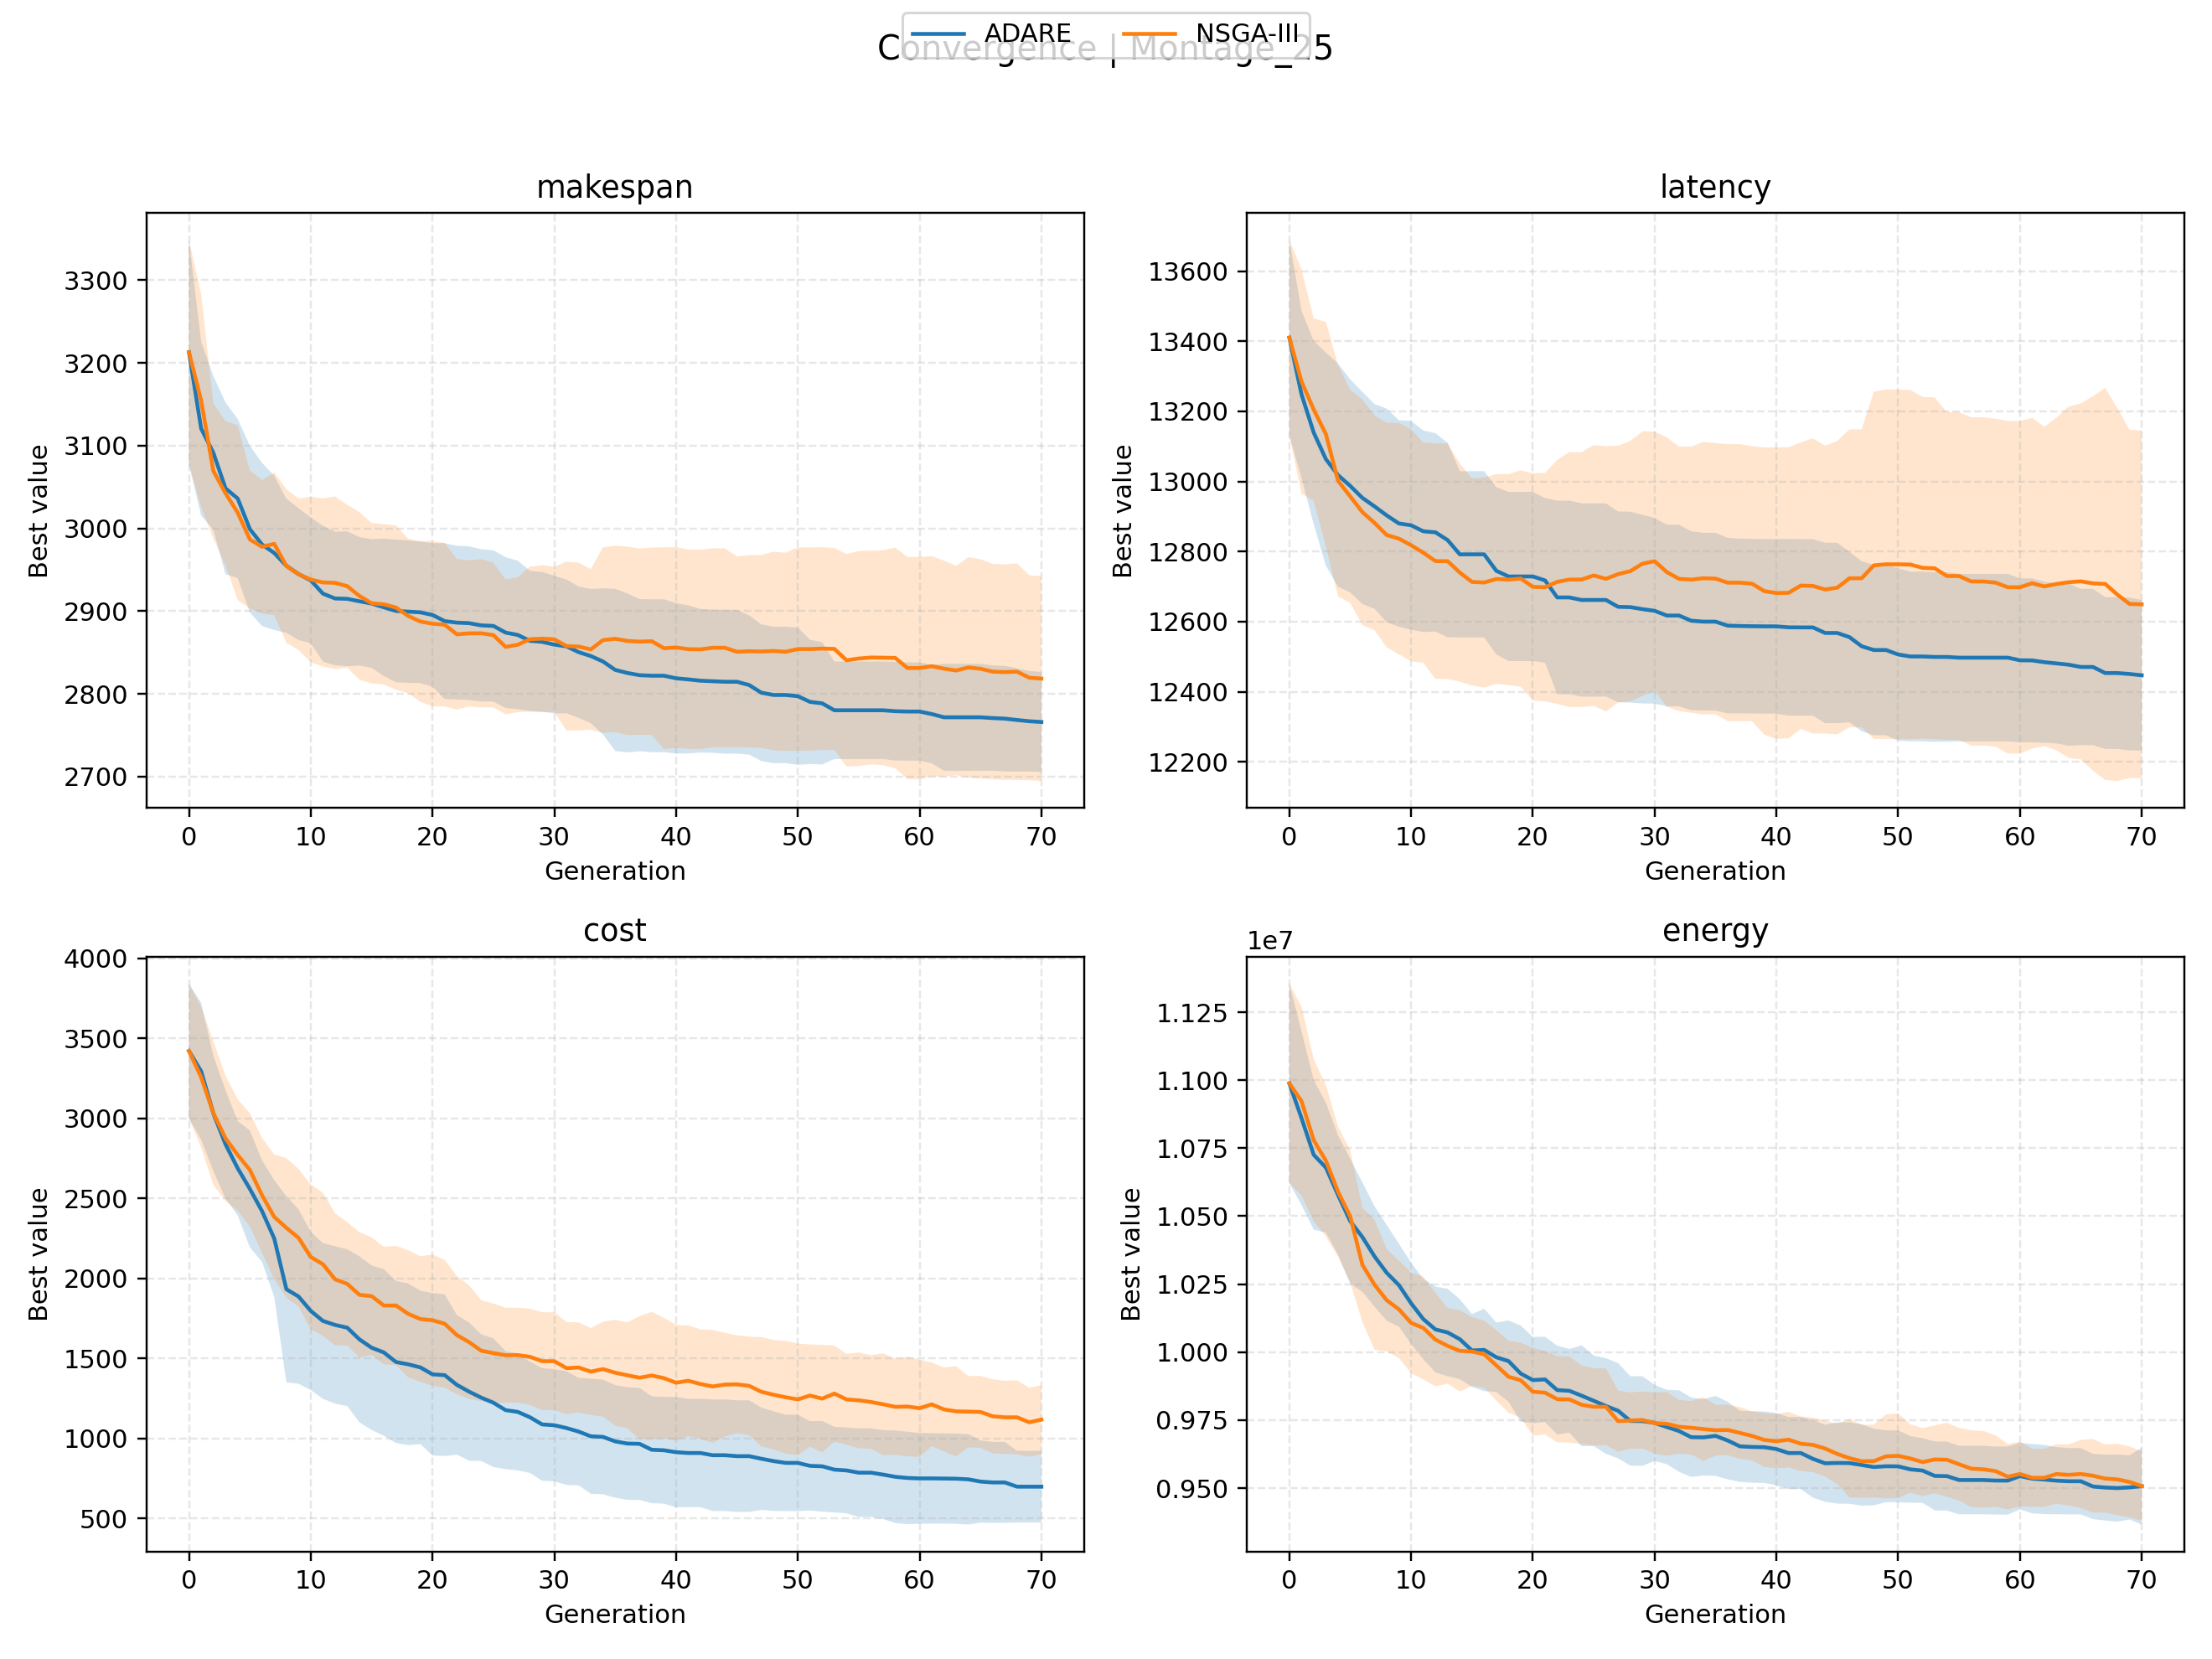
\includegraphics[width=\linewidth]{convergence_test_montage25.png}\\[-0.5ex]
\scriptsize (a) Montage\_25
\end{minipage}\hfill
\begin{minipage}[t]{0.48\textwidth}
\centering
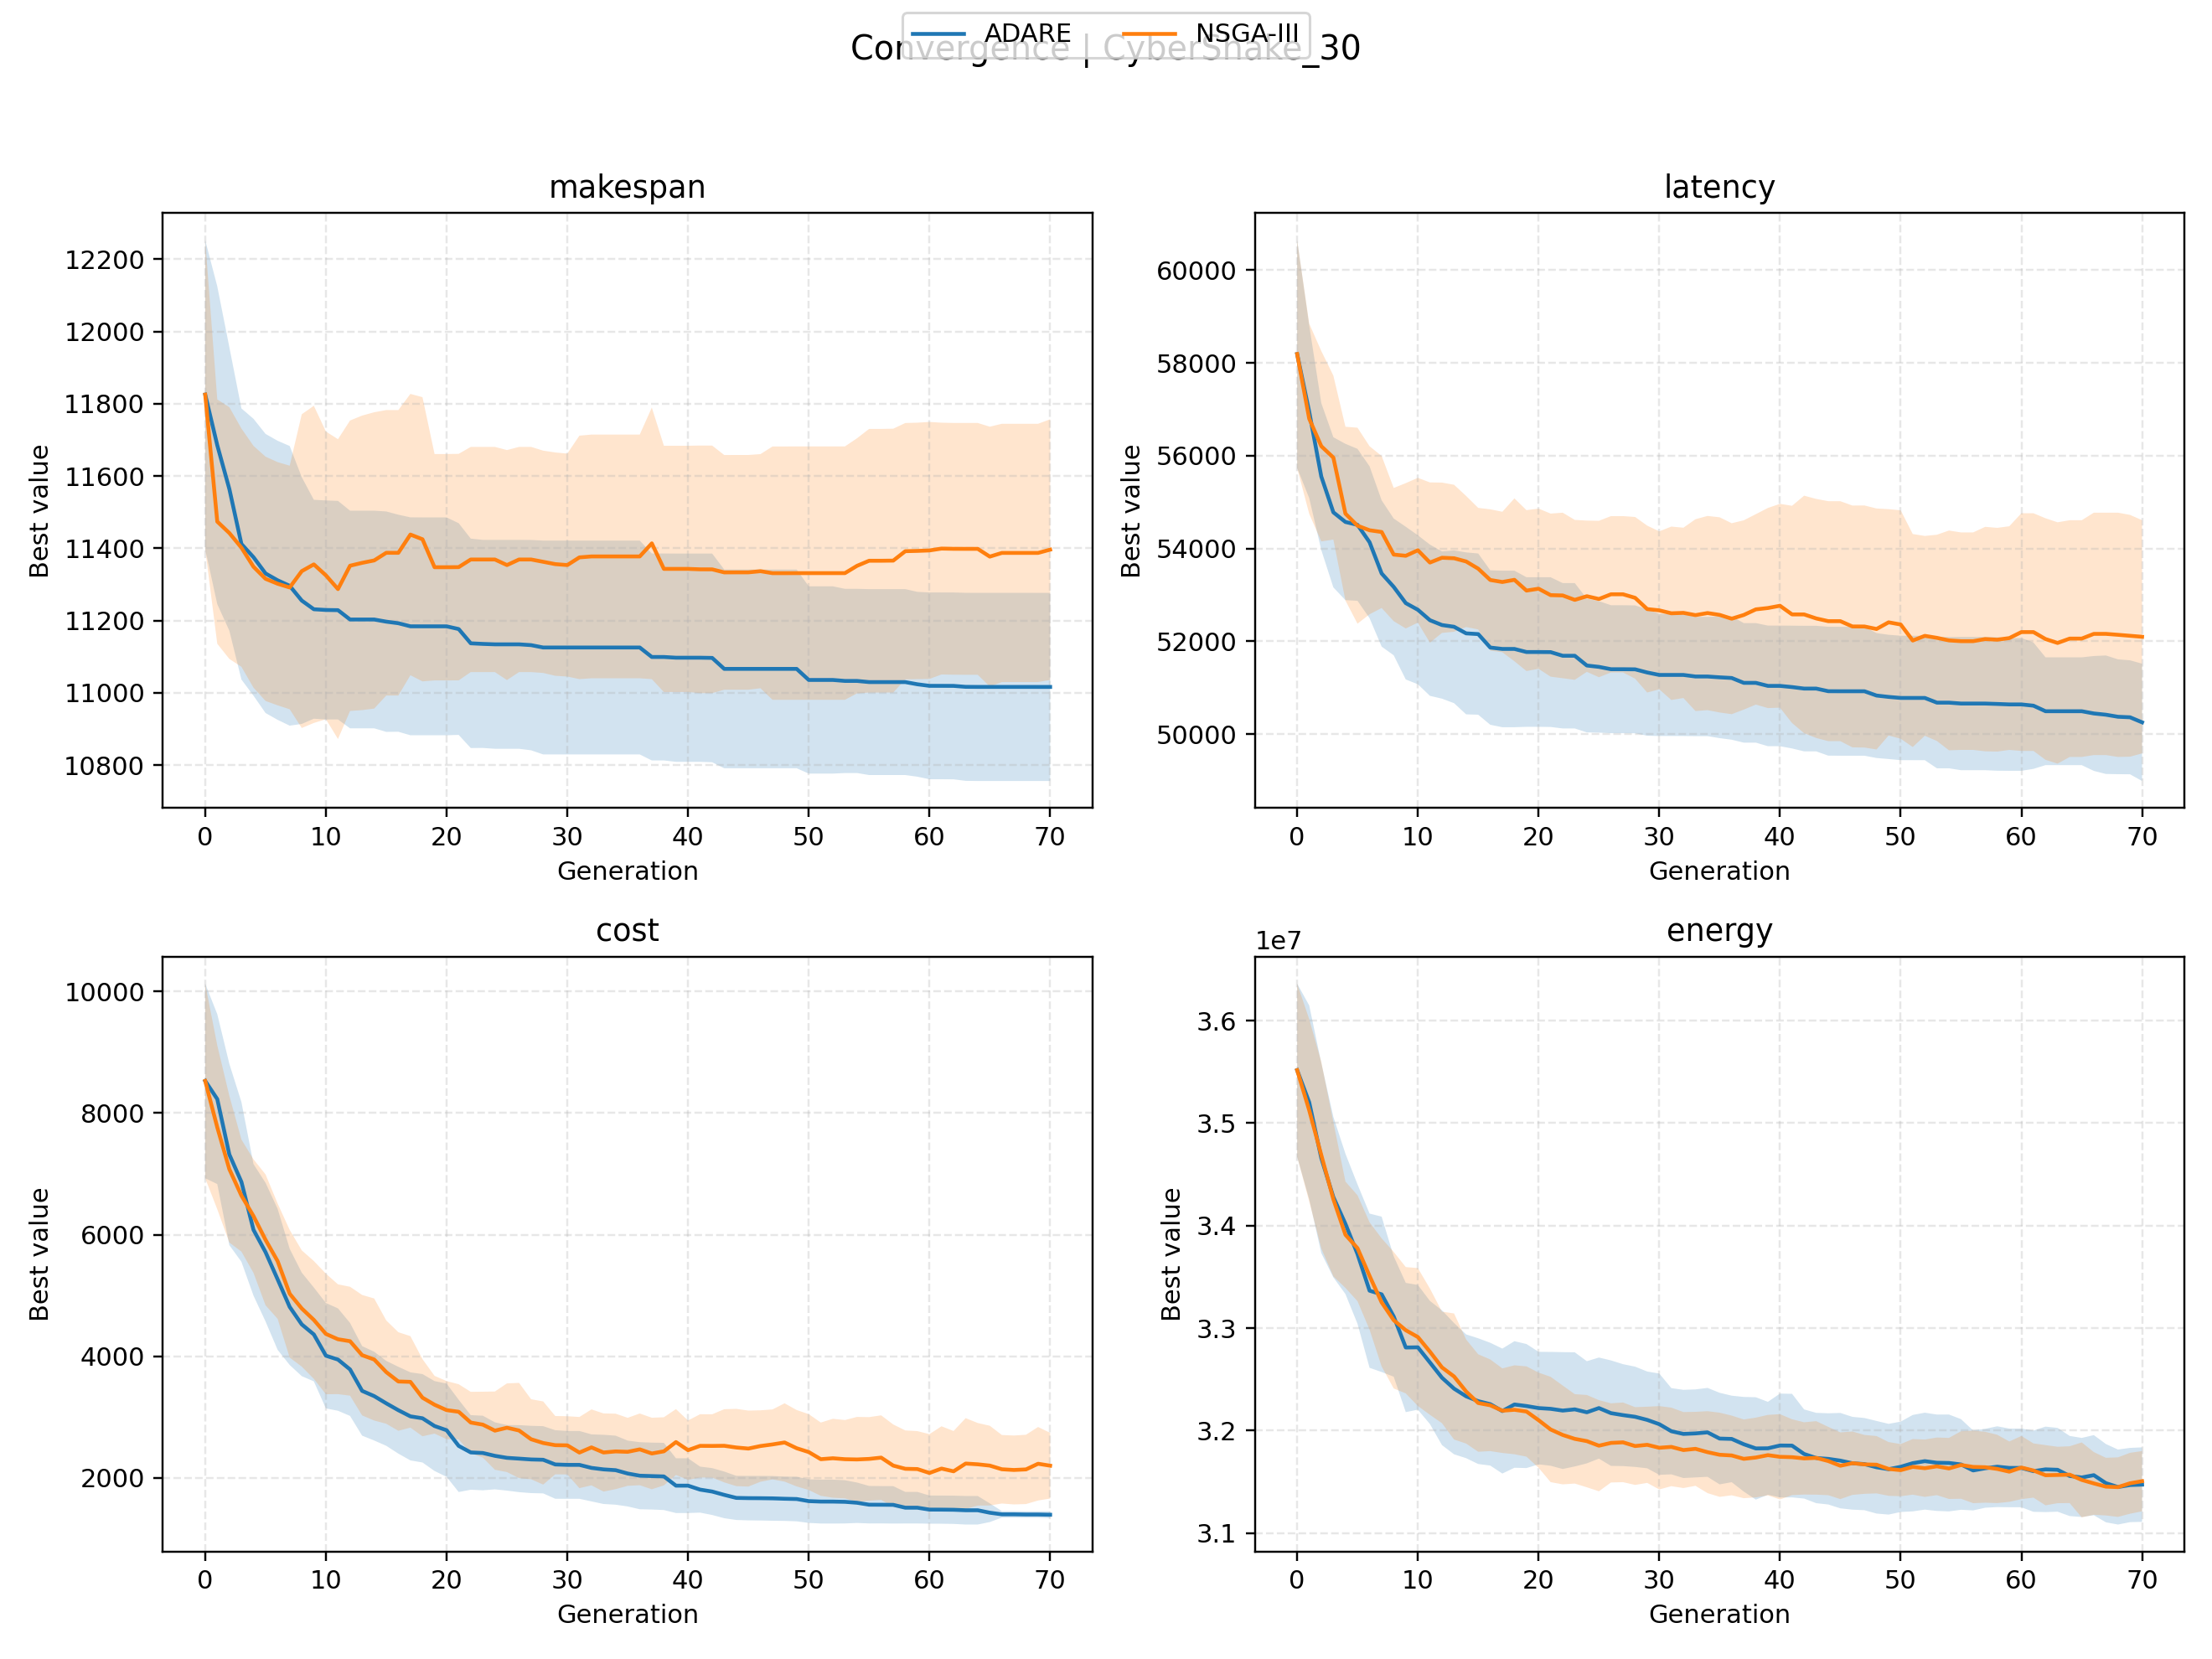
\includegraphics[width=\linewidth]{convergence_test_cybershake30.png}\\[-0.5ex]
\scriptsize (b) CyberShake\_30
\end{minipage}

\vspace{0.6ex}

\begin{minipage}[t]{0.68\textwidth}
\centering
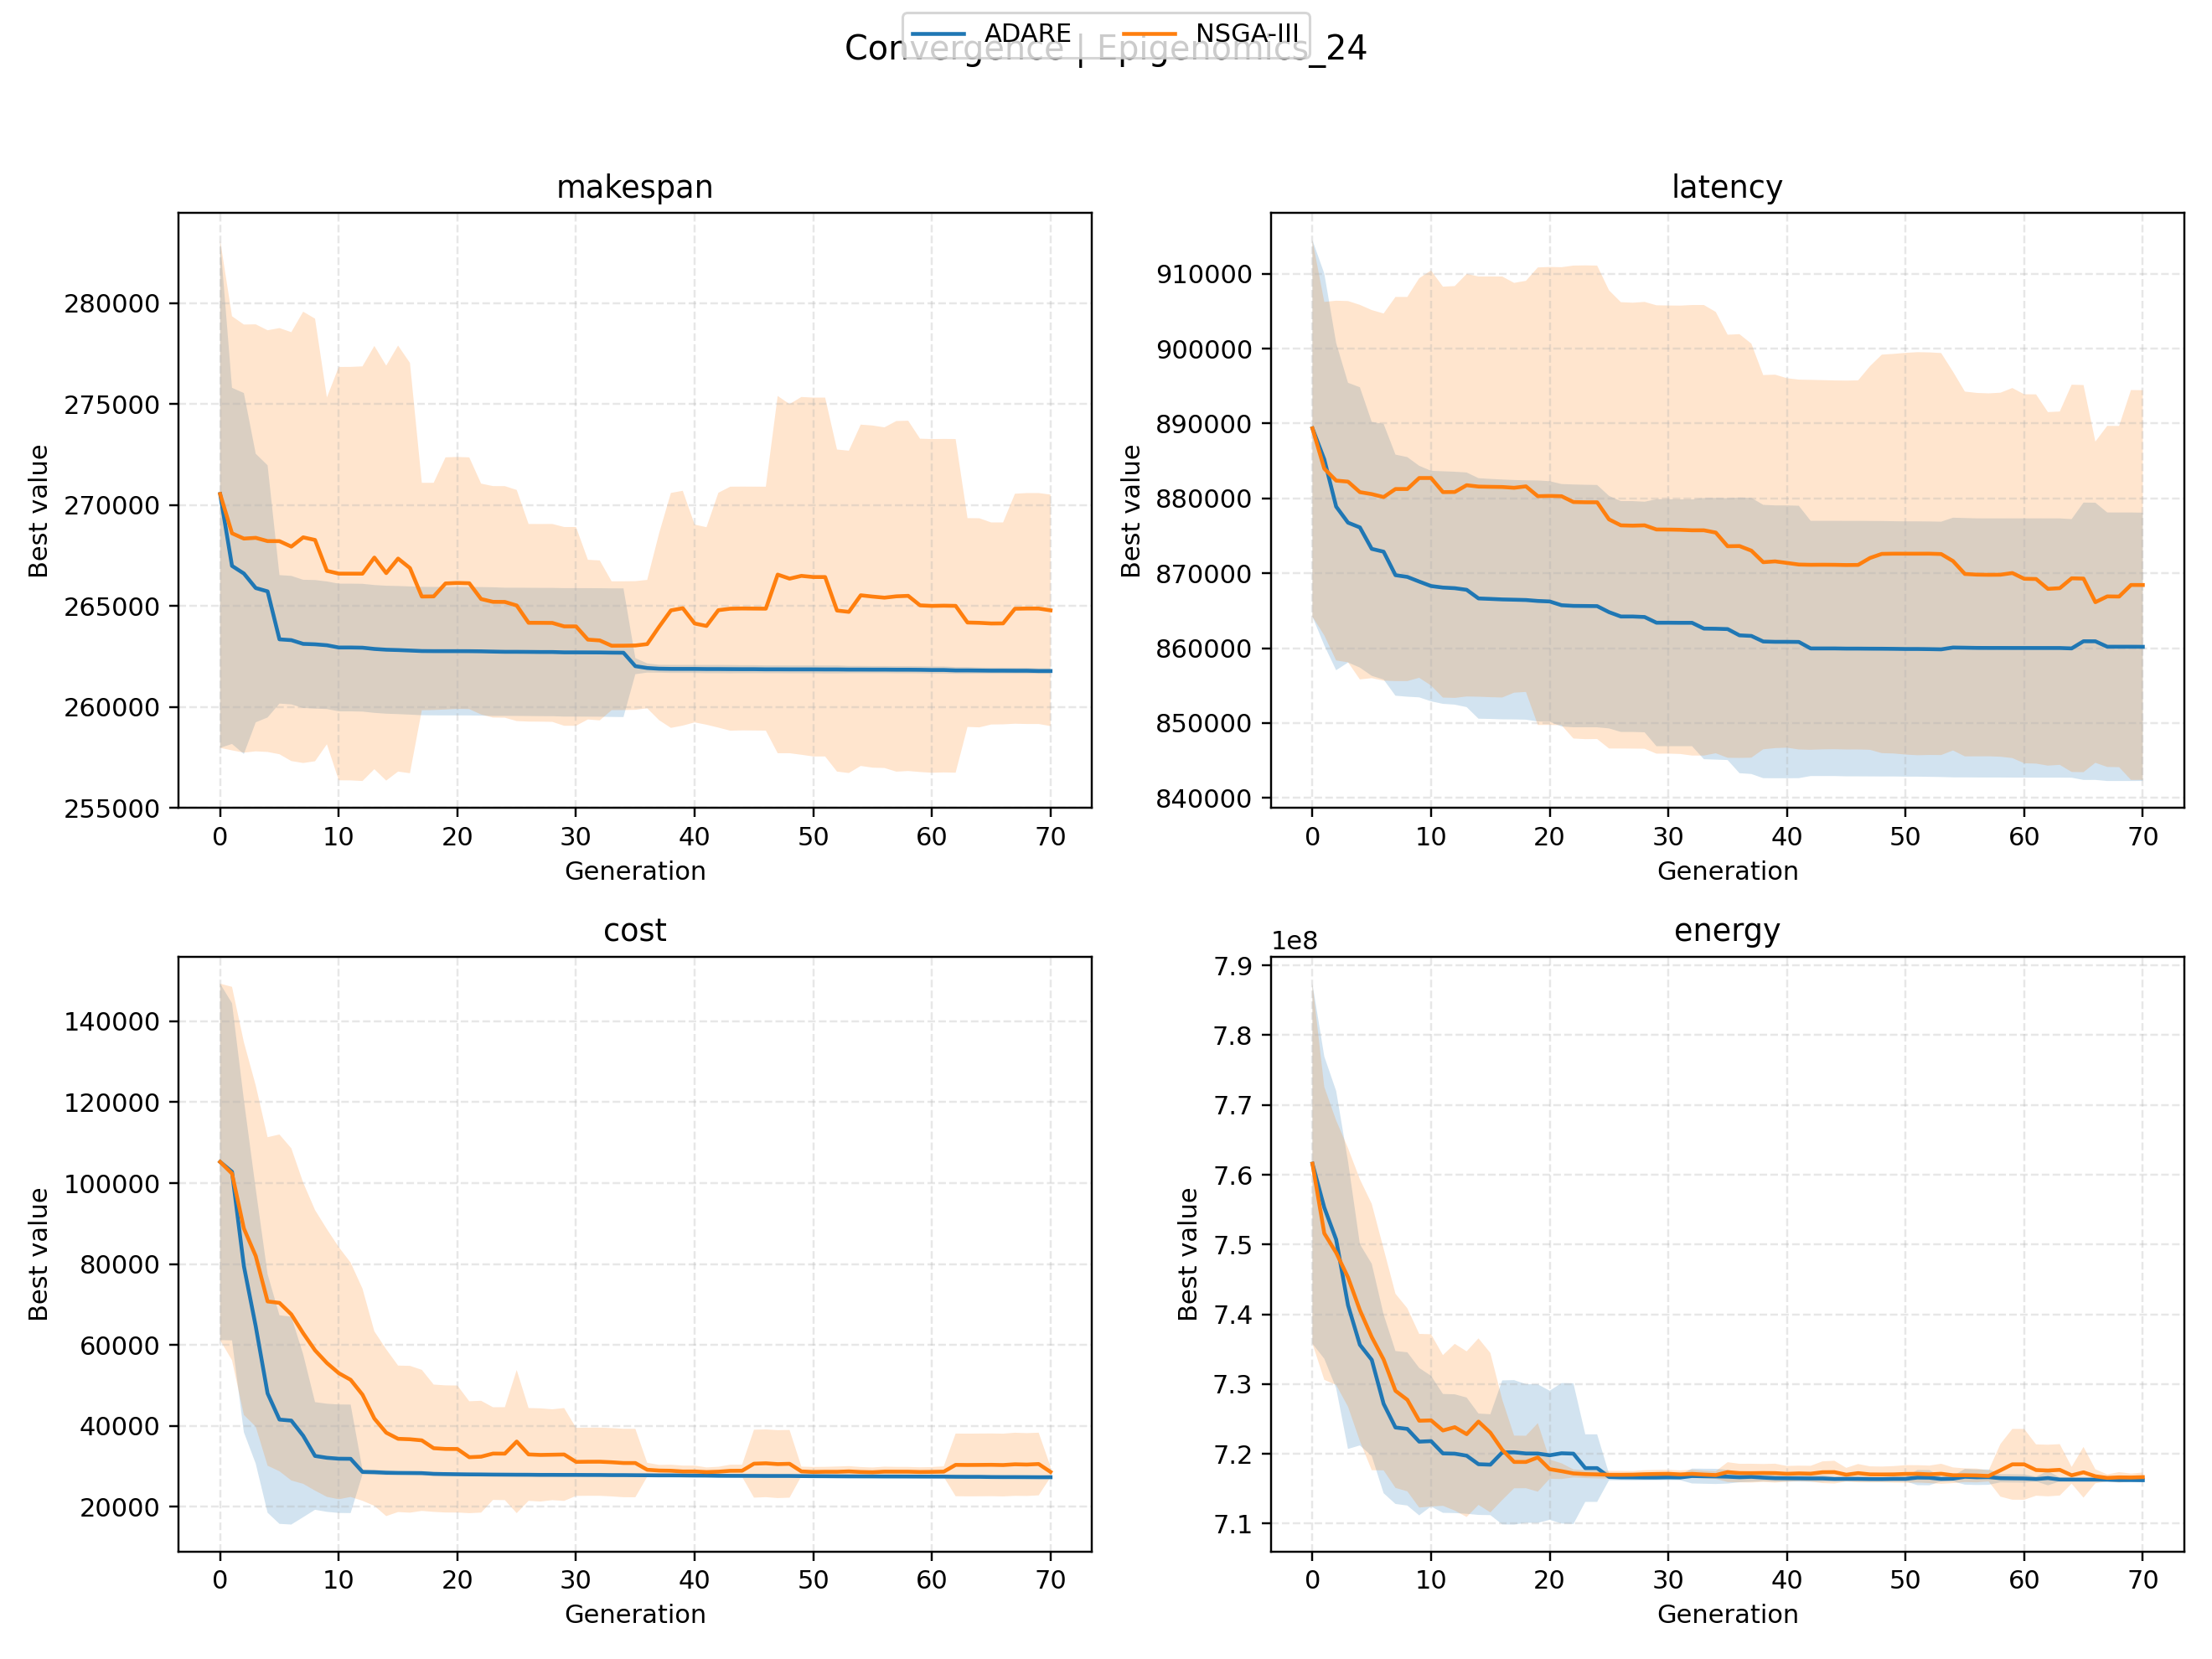
\includegraphics[width=\linewidth]{convergence_test_epigenomics24.png}\\[-0.5ex]
\scriptsize (c) Epigenomics\_24
\end{minipage}
\caption{Convergence traces (best objective values by generation) for Montage, CyberShake, and Epigenomics. Larger panels are used to improve readability of generation-wise trajectories and confidence bands.}
\label{fig:conv_all}
\end{figure}

Figure~\ref{fig:conv_all} supports the control interpretation of ADARE: the method changes search dynamics, not only final fronts. The effect is strongest on Montage and CyberShake, while Epigenomics benefits more through structural front quality than through large runtime gains.

These empirical observations now motivate a deeper discussion of why static NSGA-III underperforms in heterogeneous environments and how ADARE's design choices affect robustness.
\section{Discussion}
\subsection{Why Static NSGA-III Underperforms in Heterogeneous Environments}
The central failure mode of a static NSGA-III pipeline in our setting is not the selection operator itself. NSGA-III's reference-point mechanism remains strong. The problem lies in \emph{operator control rigidity}: a fixed crossover/mutation schedule assumes a stable reward landscape, whereas workflow scheduling over heterogeneous edge/fog/cloud resources exhibits phase changes during search.

Early generations require broad exploration to discover useful task-node assignments under precedence and bandwidth constraints. Later generations benefit from operators that preserve structure and refine local trade-offs. A static schedule cannot express this shift explicitly, while ADARE's online controller does so implicitly by updating operator preference from observed rewards.

\subsection{Justification of Experimental Choices}
\paragraph{Population size and generation count.}
We use population size 100 and 70 generations to keep comparisons computationally affordable on a local workstation while preserving enough diversity for four-objective optimization. Increasing population size improves front coverage but raises evaluator cost superlinearly in practice through more offspring evaluations and archive processing. The chosen configuration is a compromise between statistical replication and per-run search depth.

\paragraph{Seeding and fairness.}
Seed control is not a cosmetic choice. In stochastic MOEAs, comparing unmatched runs can confound algorithmic differences with initialization variance. Our paired design uses the same initial population for ADARE and NSGA-III for every run, which makes Wilcoxon and Cliff's delta more informative.

\paragraph{Why 20 runs.}
The original artifact analysis used 6 runs, which is often enough to identify strong effects but remains fragile for borderline metrics (e.g., runtime on Epigenomics or IGD on some benchmarks). We moved to 20 paired runs to stabilize mean estimates and effect sizes. The contrast between strong and weak effects in Table~\ref{tab:stats20} demonstrates why this matters: some improvements remain visible but become statistically weaker once variance is better sampled.

\subsection{Sensitivity and Robustness Trends}
Our observations suggest three sensitivity patterns.
\begin{enumerate}
    \item \textbf{Run count sensitivity}: metrics with small effect sizes (notably runtime on Epigenomics and IGD on Montage/Epigenomics) are sensitive to the number of repetitions and should not be interpreted from very small samples.
    \item \textbf{Mutation/Archive sensitivity}: ADARE's strongest empirical gains are associated with spacing, coverage, and objective extremes, indicating that density-aware mutation and archive guidance dominate the observed improvements in difficult landscapes.
    \item \textbf{Benchmark dependence}: ADARE delivers the clearest quality/runtime improvements on CyberShake and Montage, while Epigenomics exhibits a more nuanced trade-off (strong spacing/coverage gains, weaker runtime significance).
\end{enumerate}

These patterns support the adaptive-control interpretation: ADARE is not uniformly superior on every metric, but it improves the overall search behavior in a way that is consistent with the benchmark's structural difficulty.

\subsection{Limitations and Artifact Scope}
Two limitations should be stated explicitly. First, the current artifact directly implements NSGA-III as the paired baseline; NSGA-II and MOEA/D are included in our comparative positioning but not yet re-implemented under the same evaluator in this code snapshot. Second, while we provide the required V1--V5 ablation protocol and variant mapping, the full 20-run ablation sweep is deferred to a dedicated camera-ready artifact extension because it substantially expands total runtime on a local workstation.

These limitations do not affect the validity of the main ADARE-vs-NSGA-III comparison, but they do define the next engineering steps toward a broader benchmark suite.

\section{Conclusion}
We reframed ADARE as a \emph{learning-guided adaptive control mechanism} for many-objective workflow scheduling, rather than as a simple scheduler variant. This framing is technically useful: it clarifies why online learning (operator control) belongs at the center of the method, and why the evolutionary backbone can remain largely unchanged.

Under a fairness-controlled protocol (same initialization, same budget, same evaluator) and a strengthened statistical setup (20 paired runs per benchmark), ADARE improves overall many-objective search quality and runtime against NSGA-III on three heterogeneous workflow instances. The gains are strongest in HV, coverage, spacing, and objective extremes, with CyberShake showing the clearest combined benefit. Importantly, the measured control overhead remains near 5\% on average, which preserves system practicality.

For the ECML PKDD research framing, the main message is therefore simple: workflow scheduling in heterogeneous distributed systems can be improved by treating evolutionary operator choice as an \emph{online learning control problem}. Future work will complete the 20-run V1--V5 ablation sweep and extend the artifact with directly implemented NSGA-II and MOEA/D baselines under the same evaluator.

\begin{thebibliography}{99}
\bibitem{topcuoglu2002heft}
Topcuoglu, H., Hariri, S., Wu, M.-Y.: Performance-effective and low-complexity task scheduling for heterogeneous computing. IEEE Transactions on Parallel and Distributed Systems \textbf{13}(3), 260--274 (2002)

\bibitem{bonomi2012fog}
Bonomi, F., Milito, R., Zhu, J., Addepalli, S.: Fog computing and its role in the Internet of Things. In: MCC Workshop on Mobile Cloud Computing, pp.~13--16 (2012)

\bibitem{deb2002nsga2}
Deb, K., Pratap, A., Agarwal, S., Meyarivan, T.: A fast and elitist multiobjective genetic algorithm: NSGA-II. IEEE Transactions on Evolutionary Computation \textbf{6}(2), 182--197 (2002)

\bibitem{zhang2007moead}
Zhang, Q., Li, H.: MOEA/D: A multiobjective evolutionary algorithm based on decomposition. IEEE Transactions on Evolutionary Computation \textbf{11}(6), 712--731 (2007)

\bibitem{coleman2021wfcommons}
Coleman, T., Babuji, Y., Li, H., et al.: WfCommons: A framework for enabling scientific workflow research and development. Scientific Data \textbf{9}, 220 (2022).

\bibitem{deb2014nsga3}
Deb, K., Jain, H.: An evolutionary many-objective optimization algorithm using reference-point-based nondominated sorting approach, part I: Solving problems with box constraints. IEEE Transactions on Evolutionary Computation \textbf{18}(4), 577--601 (2014)

\bibitem{auer2002ucb}
Auer, P., Cesa-Bianchi, N., Fischer, P.: Finite-time analysis of the multiarmed bandit problem. Machine Learning \textbf{47}, 235--256 (2002)

\bibitem{besbes2014nonstationary}
Besbes, O., Gur, Y., Zeevi, A.: Stochastic multi-armed-bandit problem with non-stationary rewards. In: Advances in Neural Information Processing Systems (NeurIPS), vol.~27 (2014)

\bibitem{jiao2023ovea}
Jiao, K., Chen, J., Xin, B., Li, L.: OVEA: A reference vector based multiobjective evolutionary algorithm with Q-learning for operator adaptation. Evolutionary Computation \textbf{31}(3), 375--400 (2023)

\bibitem{song2024survey}
Song, A., Wang, J., Li, K., Zhang, Q.: Reinforcement learning-assisted evolutionary algorithm: A survey and research opportunities. ACM Computing Surveys \textbf{56}(12), Article 311 (2024)

\bibitem{wang2025mrlmoea}
Wang, K., Wang, Y., Xie, X., Yu, S., Zhang, Q.: MRL-MOEA: Multi-role learning based many-objective evolutionary algorithm. Scientific Reports \textbf{15}, 25039 (2025)

\bibitem{xue2025qlmoead}
Xue, J., Yang, S., Zhao, X., Hu, Y.: QLMOEA/D-AWA: A Q-learning-based decomposition multi-objective optimization evolutionary algorithm with adaptive weight adjustment. Scientific Reports \textbf{15}, 17290 (2025)

\bibitem{cui2026drlmmea}
Cui, W., Song, A., Wang, J., Zhang, Q.: DRLMMEA: Deep reinforcement learning-assisted many-objective evolutionary algorithm. Nature Communications \textbf{17}, 1084 (2026)

\bibitem{mao2017mecsurvey}
Mao, Y., You, C., Zhang, J., Huang, K., Letaief, K.B.: A survey on mobile edge computing: The communication perspective. IEEE Communications Surveys \& Tutorials \textbf{19}(4), 2322--2358 (2017)

\bibitem{wilcoxon1945}
Wilcoxon, F.: Individual comparisons by ranking methods. Biometrics Bulletin \textbf{1}(6), 80--83 (1945)

\bibitem{cliff1993}
Cliff, N.: Dominance statistics: Ordinal analyses to answer ordinal questions. Psychological Bulletin \textbf{114}(3), 494--509 (1993)

\bibitem{karafotias2015parameter}
Karafotias, G., Hoogendoorn, M., Eiben, A.E.: Parameter control in evolutionary algorithms: Trends and challenges. IEEE Transactions on Evolutionary Computation \textbf{19}(2), 167--187 (2015)

\bibitem{coello2007emo}
Coello Coello, C.A., Lamont, G.B., Van Veldhuizen, D.A.: Evolutionary Algorithms for Solving Multi-Objective Problems, 2nd edn. Springer (2007)

\bibitem{pegasus}
Deelman, E., Singh, G., Su, M.-H., et al.: Pegasus: A framework for mapping complex scientific workflows onto distributed systems. Scientific Programming \textbf{13}(3), 219--237 (2005)

\bibitem{wfcommonsrepo}
WfCommons Project: WfCommons: benchmark instances and workflow tools. \url{https://wfcommons.org/} (accessed February 24, 2026)

\end{thebibliography}

\end{document}

